\section{Reduced-form evidence}\label{sec:reduced_form}

In this section, we confirm the empirical relevance of LOP deviations and choice set differences as margins of geographic market segmentation. We confirm that price differences for identical product varieties are larger across international region pairs compared to intranational pairs. Importantly, there are also substantial differences in the set of barcodes and firms that are commonly available to consumers between intranational and international pairs. 

\subsection{LOP Deviations}
To compute LOP deviations, we first aggregate the data to the product variety-NUTS2 region-year level and by computing average prices within each cell. Then, we compute for each product variety purchased in a given year the log price differences between all NUTS2 region pairs for which there exists a price observation in both regions. Figure \ref{fig: app_redform_dp_unw_p} shows that the distribution of LOP deviations is centered around zero with most mass falling in between $-0.25$ and $0.25$ log points. To understand whether LOP deviations are larger across international region pairs versus intranational pairs, we compute the standard deviation LOP deviations within product category-region pair-year cells across product varieties.\footnote{In contrast to \citet{Gopinath2011} and \citet{Beck2020} who focus on absolute log price deviations, we choose to compute standard deviations as the measure of dispersion to be consistent with section \ref{sec:border_effects_eu}.} Figure \ref{fig: redform_lop} shows the conditional distribution of the standard deviations for international pairs in red and intranational region pairs in gray. Price dispersion is larger for international region pairs as the conditional distribution for international pairs as both its mode and tail are shifted to the right compared to the distribution for intranational pairs. While a little under 70\% of LOP deviations fall between $[-0.124,0.124]$ for intranational pairs, this spread rises to $[-0.281,0.281]$ for international pairs.

\begin{figure}[H]
    \centering
    \caption{Standard deviation of LOP deviations}
    \label{fig: redform_lop}
    \scalebox{0.90}{% Created by tikzDevice version 0.12.3.1 on 2022-10-03 21:34:35
% !TEX encoding = UTF-8 Unicode
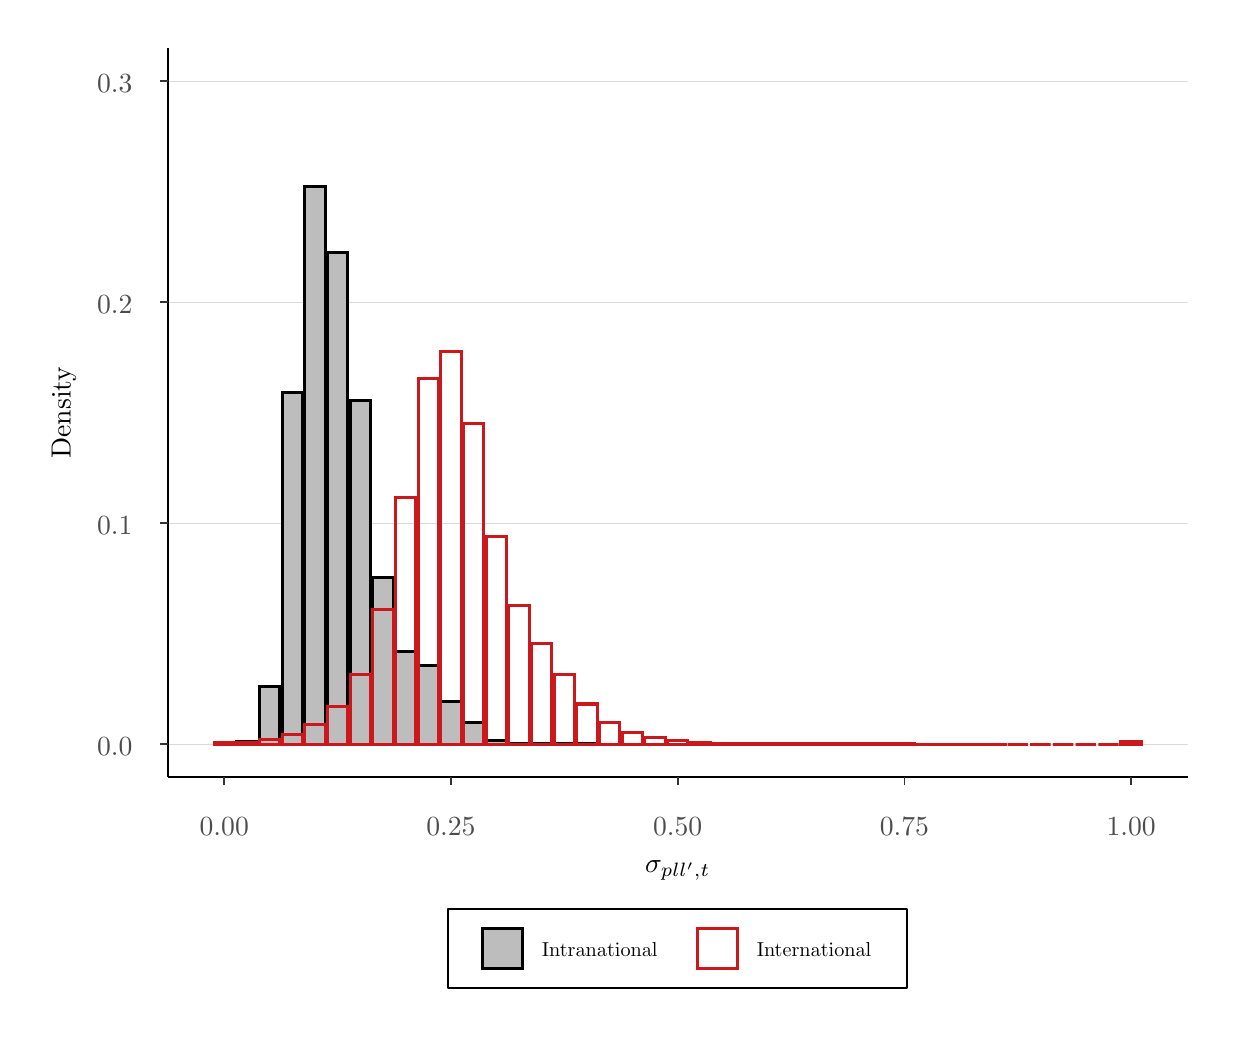
\begin{tikzpicture}[x=1pt,y=1pt]
\definecolor{fillColor}{RGB}{255,255,255}
\path[use as bounding box,fill=fillColor,fill opacity=0.00] (0,0) rectangle (433.62,361.35);
\begin{scope}
\path[clip] (  0.00,  0.00) rectangle (433.62,361.35);
\definecolor{drawColor}{RGB}{255,255,255}
\definecolor{fillColor}{RGB}{255,255,255}

\path[draw=drawColor,line width= 0.6pt,line join=round,line cap=round,fill=fillColor] (  0.00,  0.00) rectangle (433.62,361.35);
\end{scope}
\begin{scope}
\path[clip] ( 50.59, 90.50) rectangle (419.17,354.12);
\definecolor{drawColor}{RGB}{255,255,255}

\path[draw=drawColor,line width= 0.3pt,line join=round] ( 50.59,142.42) --
	(419.17,142.42);

\path[draw=drawColor,line width= 0.3pt,line join=round] ( 50.59,222.31) --
	(419.17,222.31);

\path[draw=drawColor,line width= 0.3pt,line join=round] ( 50.59,302.20) --
	(419.17,302.20);

\path[draw=drawColor,line width= 0.3pt,line join=round] (111.99, 90.50) --
	(111.99,354.12);

\path[draw=drawColor,line width= 0.3pt,line join=round] (193.92, 90.50) --
	(193.92,354.12);

\path[draw=drawColor,line width= 0.3pt,line join=round] (275.84, 90.50) --
	(275.84,354.12);

\path[draw=drawColor,line width= 0.3pt,line join=round] (357.76, 90.50) --
	(357.76,354.12);
\definecolor{drawColor}{gray}{0.85}

\path[draw=drawColor,line width= 0.1pt,line join=round] ( 50.59,102.48) --
	(419.17,102.48);

\path[draw=drawColor,line width= 0.1pt,line join=round] ( 50.59,182.37) --
	(419.17,182.37);

\path[draw=drawColor,line width= 0.1pt,line join=round] ( 50.59,262.25) --
	(419.17,262.25);

\path[draw=drawColor,line width= 0.1pt,line join=round] ( 50.59,342.14) --
	(419.17,342.14);
\definecolor{drawColor}{RGB}{0,0,0}
\definecolor{fillColor}{gray}{0.74}

\path[draw=drawColor,line width= 1.1pt,line cap=rect,fill=fillColor] ( 67.34,102.48) rectangle ( 74.72,102.49);
\definecolor{drawColor}{RGB}{203,24,29}

\path[draw=drawColor,line width= 1.1pt,line cap=rect] ( 67.34,102.48) rectangle ( 74.72,103.04);
\definecolor{drawColor}{RGB}{0,0,0}

\path[draw=drawColor,line width= 1.1pt,line cap=rect,fill=fillColor] ( 75.54,102.48) rectangle ( 82.91,103.47);
\definecolor{drawColor}{RGB}{203,24,29}

\path[draw=drawColor,line width= 1.1pt,line cap=rect] ( 75.54,102.48) rectangle ( 82.91,103.21);
\definecolor{drawColor}{RGB}{0,0,0}

\path[draw=drawColor,line width= 1.1pt,line cap=rect,fill=fillColor] ( 83.73,102.48) rectangle ( 91.10,123.42);
\definecolor{drawColor}{RGB}{203,24,29}

\path[draw=drawColor,line width= 1.1pt,line cap=rect] ( 83.73,102.48) rectangle ( 91.10,104.17);
\definecolor{drawColor}{RGB}{0,0,0}

\path[draw=drawColor,line width= 1.1pt,line cap=rect,fill=fillColor] ( 91.92,102.48) rectangle ( 99.29,229.43);
\definecolor{drawColor}{RGB}{203,24,29}

\path[draw=drawColor,line width= 1.1pt,line cap=rect] ( 91.92,102.48) rectangle ( 99.29,106.05);
\definecolor{drawColor}{RGB}{0,0,0}

\path[draw=drawColor,line width= 1.1pt,line cap=rect,fill=fillColor] (100.11,102.48) rectangle (107.49,303.89);
\definecolor{drawColor}{RGB}{203,24,29}

\path[draw=drawColor,line width= 1.1pt,line cap=rect] (100.11,102.48) rectangle (107.49,109.59);
\definecolor{drawColor}{RGB}{0,0,0}

\path[draw=drawColor,line width= 1.1pt,line cap=rect,fill=fillColor] (108.31,102.48) rectangle (115.68,279.94);
\definecolor{drawColor}{RGB}{203,24,29}

\path[draw=drawColor,line width= 1.1pt,line cap=rect] (108.31,102.48) rectangle (115.68,116.13);
\definecolor{drawColor}{RGB}{0,0,0}

\path[draw=drawColor,line width= 1.1pt,line cap=rect,fill=fillColor] (116.50,102.48) rectangle (123.87,226.48);
\definecolor{drawColor}{RGB}{203,24,29}

\path[draw=drawColor,line width= 1.1pt,line cap=rect] (116.50,102.48) rectangle (123.87,127.75);
\definecolor{drawColor}{RGB}{0,0,0}

\path[draw=drawColor,line width= 1.1pt,line cap=rect,fill=fillColor] (124.69,102.48) rectangle (132.06,162.75);
\definecolor{drawColor}{RGB}{203,24,29}

\path[draw=drawColor,line width= 1.1pt,line cap=rect] (124.69,102.48) rectangle (132.06,150.95);
\definecolor{drawColor}{RGB}{0,0,0}

\path[draw=drawColor,line width= 1.1pt,line cap=rect,fill=fillColor] (132.88,102.48) rectangle (140.26,135.87);
\definecolor{drawColor}{RGB}{203,24,29}

\path[draw=drawColor,line width= 1.1pt,line cap=rect] (132.88,102.48) rectangle (140.26,191.43);
\definecolor{drawColor}{RGB}{0,0,0}

\path[draw=drawColor,line width= 1.1pt,line cap=rect,fill=fillColor] (141.08,102.48) rectangle (148.45,130.98);
\definecolor{drawColor}{RGB}{203,24,29}

\path[draw=drawColor,line width= 1.1pt,line cap=rect] (141.08,102.48) rectangle (148.45,234.56);
\definecolor{drawColor}{RGB}{0,0,0}

\path[draw=drawColor,line width= 1.1pt,line cap=rect,fill=fillColor] (149.27,102.48) rectangle (156.64,118.01);
\definecolor{drawColor}{RGB}{203,24,29}

\path[draw=drawColor,line width= 1.1pt,line cap=rect] (149.27,102.48) rectangle (156.64,244.44);
\definecolor{drawColor}{RGB}{0,0,0}

\path[draw=drawColor,line width= 1.1pt,line cap=rect,fill=fillColor] (157.46,102.48) rectangle (164.83,110.40);
\definecolor{drawColor}{RGB}{203,24,29}

\path[draw=drawColor,line width= 1.1pt,line cap=rect] (157.46,102.48) rectangle (164.83,218.22);
\definecolor{drawColor}{RGB}{0,0,0}

\path[draw=drawColor,line width= 1.1pt,line cap=rect,fill=fillColor] (165.65,102.48) rectangle (173.03,103.67);
\definecolor{drawColor}{RGB}{203,24,29}

\path[draw=drawColor,line width= 1.1pt,line cap=rect] (165.65,102.48) rectangle (173.03,177.58);
\definecolor{drawColor}{RGB}{0,0,0}

\path[draw=drawColor,line width= 1.1pt,line cap=rect,fill=fillColor] (173.85,102.48) rectangle (181.22,102.67);
\definecolor{drawColor}{RGB}{203,24,29}

\path[draw=drawColor,line width= 1.1pt,line cap=rect] (173.85,102.48) rectangle (181.22,152.40);
\definecolor{drawColor}{RGB}{0,0,0}

\path[draw=drawColor,line width= 1.1pt,line cap=rect,fill=fillColor] (182.04,102.48) rectangle (189.41,102.55);
\definecolor{drawColor}{RGB}{203,24,29}

\path[draw=drawColor,line width= 1.1pt,line cap=rect] (182.04,102.48) rectangle (189.41,138.73);
\definecolor{drawColor}{RGB}{0,0,0}

\path[draw=drawColor,line width= 1.1pt,line cap=rect,fill=fillColor] (190.23,102.48) rectangle (197.60,102.53);
\definecolor{drawColor}{RGB}{203,24,29}

\path[draw=drawColor,line width= 1.1pt,line cap=rect] (190.23,102.48) rectangle (197.60,127.48);
\definecolor{drawColor}{RGB}{0,0,0}

\path[draw=drawColor,line width= 1.1pt,line cap=rect,fill=fillColor] (198.42,102.48) rectangle (205.80,102.50);
\definecolor{drawColor}{RGB}{203,24,29}

\path[draw=drawColor,line width= 1.1pt,line cap=rect] (198.42,102.48) rectangle (205.80,116.95);
\definecolor{drawColor}{RGB}{0,0,0}

\path[draw=drawColor,line width= 1.1pt,line cap=rect,fill=fillColor] (206.61,102.48) rectangle (213.99,102.48);
\definecolor{drawColor}{RGB}{203,24,29}

\path[draw=drawColor,line width= 1.1pt,line cap=rect] (206.61,102.48) rectangle (213.99,110.25);
\definecolor{drawColor}{RGB}{0,0,0}

\path[draw=drawColor,line width= 1.1pt,line cap=rect,fill=fillColor] (214.81,102.48) rectangle (222.18,102.48);
\definecolor{drawColor}{RGB}{203,24,29}

\path[draw=drawColor,line width= 1.1pt,line cap=rect] (214.81,102.48) rectangle (222.18,106.79);
\definecolor{drawColor}{RGB}{0,0,0}

\path[draw=drawColor,line width= 1.1pt,line cap=rect,fill=fillColor] (223.00,102.48) rectangle (230.37,102.48);
\definecolor{drawColor}{RGB}{203,24,29}

\path[draw=drawColor,line width= 1.1pt,line cap=rect] (223.00,102.48) rectangle (230.37,104.83);
\definecolor{drawColor}{RGB}{0,0,0}

\path[draw=drawColor,line width= 1.1pt,line cap=rect,fill=fillColor] (231.19,102.48) rectangle (238.56,102.48);
\definecolor{drawColor}{RGB}{203,24,29}

\path[draw=drawColor,line width= 1.1pt,line cap=rect] (231.19,102.48) rectangle (238.56,103.70);
\definecolor{drawColor}{RGB}{0,0,0}

\path[draw=drawColor,line width= 1.1pt,line cap=rect,fill=fillColor] (239.38,102.48) rectangle (246.76,102.48);
\definecolor{drawColor}{RGB}{203,24,29}

\path[draw=drawColor,line width= 1.1pt,line cap=rect] (239.38,102.48) rectangle (246.76,103.13);
\definecolor{drawColor}{RGB}{0,0,0}

\path[draw=drawColor,line width= 1.1pt,line cap=rect,fill=fillColor] (247.58,102.48) rectangle (254.95,102.48);
\definecolor{drawColor}{RGB}{203,24,29}

\path[draw=drawColor,line width= 1.1pt,line cap=rect] (247.58,102.48) rectangle (254.95,102.84);

\path[draw=drawColor,line width= 1.1pt,line cap=rect] (255.77,102.48) rectangle (263.14,102.71);

\path[draw=drawColor,line width= 1.1pt,line cap=rect] (263.96,102.48) rectangle (271.33,102.61);

\path[draw=drawColor,line width= 1.1pt,line cap=rect] (272.15,102.48) rectangle (279.53,102.59);

\path[draw=drawColor,line width= 1.1pt,line cap=rect] (280.35,102.48) rectangle (287.72,102.54);

\path[draw=drawColor,line width= 1.1pt,line cap=rect] (288.54,102.48) rectangle (295.91,102.53);

\path[draw=drawColor,line width= 1.1pt,line cap=rect] (296.73,102.48) rectangle (304.10,102.52);
\definecolor{drawColor}{RGB}{0,0,0}

\path[draw=drawColor,line width= 1.1pt,line cap=rect,fill=fillColor] (304.92,102.48) rectangle (312.30,102.48);
\definecolor{drawColor}{RGB}{203,24,29}

\path[draw=drawColor,line width= 1.1pt,line cap=rect] (304.92,102.48) rectangle (312.30,102.51);

\path[draw=drawColor,line width= 1.1pt,line cap=rect] (313.12,102.48) rectangle (320.49,102.50);

\path[draw=drawColor,line width= 1.1pt,line cap=rect] (321.31,102.48) rectangle (328.68,102.49);

\path[draw=drawColor,line width= 1.1pt,line cap=rect] (329.50,102.48) rectangle (336.87,102.49);

\path[draw=drawColor,line width= 1.1pt,line cap=rect] (337.69,102.48) rectangle (345.07,102.49);

\path[draw=drawColor,line width= 1.1pt,line cap=rect] (345.89,102.48) rectangle (353.26,102.49);

\path[draw=drawColor,line width= 1.1pt,line cap=rect] (354.08,102.48) rectangle (361.45,102.48);

\path[draw=drawColor,line width= 1.1pt,line cap=rect] (362.27,102.48) rectangle (369.64,102.48);

\path[draw=drawColor,line width= 1.1pt,line cap=rect] (370.46,102.48) rectangle (377.84,102.48);

\path[draw=drawColor,line width= 1.1pt,line cap=rect] (378.65,102.48) rectangle (386.03,102.48);

\path[draw=drawColor,line width= 1.1pt,line cap=rect] (386.85,102.48) rectangle (394.22,102.48);
\definecolor{drawColor}{RGB}{0,0,0}

\path[draw=drawColor,line width= 1.1pt,line cap=rect,fill=fillColor] (395.04,102.48) rectangle (402.41,102.48);
\definecolor{drawColor}{RGB}{203,24,29}

\path[draw=drawColor,line width= 1.1pt,line cap=rect] (395.04,102.48) rectangle (402.41,103.48);
\end{scope}
\begin{scope}
\path[clip] (  0.00,  0.00) rectangle (433.62,361.35);
\definecolor{drawColor}{RGB}{0,0,0}

\path[draw=drawColor,line width= 0.6pt,line join=round] ( 50.59, 90.50) --
	( 50.59,354.12);
\end{scope}
\begin{scope}
\path[clip] (  0.00,  0.00) rectangle (433.62,361.35);
\definecolor{drawColor}{gray}{0.30}

\node[text=drawColor,anchor=base east,inner sep=0pt, outer sep=0pt, scale=  1.00] at ( 37.84, 98.35) {0.0};

\node[text=drawColor,anchor=base east,inner sep=0pt, outer sep=0pt, scale=  1.00] at ( 37.84,178.23) {0.1};

\node[text=drawColor,anchor=base east,inner sep=0pt, outer sep=0pt, scale=  1.00] at ( 37.84,258.12) {0.2};

\node[text=drawColor,anchor=base east,inner sep=0pt, outer sep=0pt, scale=  1.00] at ( 37.84,338.01) {0.3};
\end{scope}
\begin{scope}
\path[clip] (  0.00,  0.00) rectangle (433.62,361.35);
\definecolor{drawColor}{gray}{0.20}

\path[draw=drawColor,line width= 0.6pt,line join=round] ( 47.84,102.48) --
	( 50.59,102.48);

\path[draw=drawColor,line width= 0.6pt,line join=round] ( 47.84,182.37) --
	( 50.59,182.37);

\path[draw=drawColor,line width= 0.6pt,line join=round] ( 47.84,262.25) --
	( 50.59,262.25);

\path[draw=drawColor,line width= 0.6pt,line join=round] ( 47.84,342.14) --
	( 50.59,342.14);
\end{scope}
\begin{scope}
\path[clip] (  0.00,  0.00) rectangle (433.62,361.35);
\definecolor{drawColor}{RGB}{0,0,0}

\path[draw=drawColor,line width= 0.6pt,line join=round] ( 50.59, 90.50) --
	(419.17, 90.50);
\end{scope}
\begin{scope}
\path[clip] (  0.00,  0.00) rectangle (433.62,361.35);
\definecolor{drawColor}{gray}{0.20}

\path[draw=drawColor,line width= 0.6pt,line join=round] ( 71.03, 87.75) --
	( 71.03, 90.50);

\path[draw=drawColor,line width= 0.6pt,line join=round] (152.95, 87.75) --
	(152.95, 90.50);

\path[draw=drawColor,line width= 0.6pt,line join=round] (234.88, 87.75) --
	(234.88, 90.50);

\path[draw=drawColor,line width= 0.6pt,line join=round] (316.80, 87.75) --
	(316.80, 90.50);

\path[draw=drawColor,line width= 0.6pt,line join=round] (398.73, 87.75) --
	(398.73, 90.50);
\end{scope}
\begin{scope}
\path[clip] (  0.00,  0.00) rectangle (433.62,361.35);
\definecolor{drawColor}{gray}{0.30}

\node[text=drawColor,anchor=base,inner sep=0pt, outer sep=0pt, scale=  1.00] at ( 71.03, 69.48) {0.00};

\node[text=drawColor,anchor=base,inner sep=0pt, outer sep=0pt, scale=  1.00] at (152.95, 69.48) {0.25};

\node[text=drawColor,anchor=base,inner sep=0pt, outer sep=0pt, scale=  1.00] at (234.88, 69.48) {0.50};

\node[text=drawColor,anchor=base,inner sep=0pt, outer sep=0pt, scale=  1.00] at (316.80, 69.48) {0.75};

\node[text=drawColor,anchor=base,inner sep=0pt, outer sep=0pt, scale=  1.00] at (398.73, 69.48) {1.00};
\end{scope}
\begin{scope}
\path[clip] (  0.00,  0.00) rectangle (433.62,361.35);
\definecolor{drawColor}{RGB}{0,0,0}

\node[text=drawColor,anchor=base,inner sep=0pt, outer sep=0pt, scale=  1.00] at (234.88, 56.13) {$\sigma_{pll',t}$};
\end{scope}
\begin{scope}
\path[clip] (  0.00,  0.00) rectangle (433.62,361.35);
\definecolor{drawColor}{RGB}{0,0,0}

\node[text=drawColor,rotate= 90.00,anchor=base,inner sep=0pt, outer sep=0pt, scale=  1.00] at ( 15.49,222.31) {Density};
\end{scope}
\begin{scope}
\path[clip] (  0.00,  0.00) rectangle (433.62,361.35);
\definecolor{drawColor}{RGB}{0,0,0}
\definecolor{fillColor}{RGB}{255,255,255}

\path[draw=drawColor,line width= 0.6pt,line join=round,line cap=round,fill=fillColor] (151.97, 14.45) rectangle (317.79, 42.80);
\end{scope}
\begin{scope}
\path[clip] (  0.00,  0.00) rectangle (433.62,361.35);

\path[] (162.97, 19.95) rectangle (180.32, 37.30);
\end{scope}
\begin{scope}
\path[clip] (  0.00,  0.00) rectangle (433.62,361.35);
\definecolor{drawColor}{RGB}{0,0,0}
\definecolor{fillColor}{gray}{0.74}

\path[draw=drawColor,line width= 1.1pt,line cap=rect,fill=fillColor] (164.39, 21.38) rectangle (178.89, 35.88);
\end{scope}
\begin{scope}
\path[clip] (  0.00,  0.00) rectangle (433.62,361.35);

\path[] (240.62, 19.95) rectangle (257.96, 37.30);
\end{scope}
\begin{scope}
\path[clip] (  0.00,  0.00) rectangle (433.62,361.35);
\definecolor{drawColor}{RGB}{203,24,29}

\path[draw=drawColor,line width= 1.1pt,line cap=rect] (242.04, 21.38) rectangle (256.54, 35.88);
\end{scope}
\begin{scope}
\path[clip] (  0.00,  0.00) rectangle (433.62,361.35);
\definecolor{drawColor}{RGB}{0,0,0}

\node[text=drawColor,anchor=base west,inner sep=0pt, outer sep=0pt, scale=  0.73] at (185.82, 25.60) {Intranational};
\end{scope}
\begin{scope}
\path[clip] (  0.00,  0.00) rectangle (433.62,361.35);
\definecolor{drawColor}{RGB}{0,0,0}

\node[text=drawColor,anchor=base west,inner sep=0pt, outer sep=0pt, scale=  0.73] at (263.46, 25.60) {International};
\end{scope}
\end{tikzpicture}
}
     \parbox{\textwidth}{
        \begin{spacing}{1} 
            {\footnotesize 
            \textit{Notes}: This figure plots the conditional distributions of the standard deviation of log LOP deviations across NUTS2-region pairs. The unit of observation is a product category-NUTS2 region pair steps. We bin the standard deviation of log price differences within product category-region pairs-year cells into 40 separate bins and compute for each bin the number of observations that fall into each bin. Finally, we winsorize the standard deviations at a standard deviation of 1.}
        \end{spacing}}
 \end{figure} 

To see whether the increased price dispersion reflects geographic market segmentation, we need to account for the fact that international region pairs are also more distant from one another compared to intranational region pairs. To this end, we follow \citet{Engel1996} and estimate: 
\begin{linenomath*}
    \begin{equation}\label{eq:border_effect_prices}
        \sigma_{pll',t} = \beta B_{ll'} + \gamma d_{ll'} + \theta_l + \theta_{l'} +
                    \lambda_{p,t} + \varepsilon_{pll',t}
    \end{equation}
\end{linenomath*}
\noindent where 

\begin{linenomath*}
    \begin{equation*}
        \sigma_{pll',t} \equiv 
            \sqrt{
                \frac{1}{N^{ll'}_{p}}
                \sum_{i \in \mathcal{B}^{ll'}_{p}} \left(\text{log}\left(p_{il',t}/p_{il,t}\right) - \widehat{\mathbb{E}_{pll',t}}\left[\text{log}\left(p_{il',t}/p_{il,t}\right)\right]
                \right)^2
            }
    \end{equation*}
\end{linenomath*}
is the standard deviation of log LOP deviations for region pair $ll'$ within product category $p$ in year $t$. We include a border dummy $B_{ll'}$ which is one when region pair $ll^{'}$ is an international pair and zero otherwise. To control for the distance between region pairs, we include $d_{ll'}$ which is the log of the population-weighted great circle distance between the regions. We focus on variation across region pairs within product category-year observations by including product category-year fixed effects. Finally, we add region fixed effects $\theta_l$ and $\theta_{l'}$ to account for the fact that certain regions might be characterized by always higher price dispersion.\footnote{Regions with disproportionally large urban centers might always have higher prices and therefore always larger price differences with any other region.}

We present the baseline OLS estimates in columns (1)-(3) of Table \ref{tab: border_effects_sd}. Column (1) shows the results when we estimate equation \ref{eq:border_effect_prices} and only include log distance $d_{ll'}$. In this case, a 100\% increase in the distance between two regions leads to a statistically significant increase in the variance of log LOP differences of 8.4ppt. In line with Figure \ref{fig: redform_lop}, column (2) shows that the standard deviation of log price differences is 15ppt larger for international pairs compared to international pairs when we only include the border dummy. Finally, in column (3) we include both distance and the border dummy. Whereas the distance effect drops considerably, the border effect remains large and precisely estimated at 15.4ppt.\footnote{Reassuringly, these border effects are quantitatively in line with the RDD estimates from \citet{Beck2020} which reports an average absolute price difference of around 18\%.} Figure \ref{fig: app_redform_sd_years} and Figure \ref{fig: app_redform_sd_cats} explore variation in the average border effect over time and across product categories respectively. In line with the results from \citet{Beck2020}, there is little systematic variation over the years. There is, however, considerably more cross-category heterogeneity. Figure \ref{fig: app_redform_sd_cats} shows that border effects estimates are significantly different from zero in all but one case and range from a low of 3.2ppt for packaged meat to a high of 42.5 for mineral water. Importantly, Figure \ref{fig: app_redform_sd_cats} also shows that while there is significant cross-sectional variation in the border effects, there is little systematic cross-category variation in LOP deviations for intranational pairs.

Columns (4) - (6) present two robustness checks. First, column (4) considers cross-country heterogeneity in the border effect. If there is substantial cross-country heterogeneity in price dispersion for intranational region pairs, \citet{Gorodnichenko2009} shows that the border effect estimate from equation \ref{eq:border_effect_prices} is contaminated with average cross-country differences in price dispersion for intranational region pairs.\footnote{This point is related to the broader issue of a simple differences-in-means regression that suffers from heterogeneous treatment effect bias under non-random treatment assignment.} To isolate the former effect, we follow \citet{Gorodnichenko2009} and augment equation \ref{eq:border_effect_prices} with country dummies that are one if region $l$ and $l'$ belong to that country and zero otherwise for all countries apart from Germany, which functions as the baseline country. In this way, the border variable $B_{ll'}$ measures the average difference in price dispersion for international region pairs relative to the average price dispersion for German intranational region pairs. The other country-specific border effects are obtained from $\beta - \gamma_{c(l)}$. Column (4) shows that the average border effect, now relative to average price dispersion for German intranational region pairs, is 12.5ppt. While the country dummies indicate that cross-country heterogeneity in price dispersion for intranational pairs exists, column (4) also shows that all border effects are positive and precisely estimated relative to average price dispersion for intranational pairs in each country. Second, in columns (5)-(6) we consider an alternative level of aggregation. To obtain the baseline results, we collapsed the retail chain dimension. However, \citet{Dellavigna2019} provides evidence that LOP deviations are much larger across chains compared to within chains. Hence, by averaging across stores, we might artificially increase price dispersion, potentially leading to an inconsistent border effect. In columns (5) and (6), we re-estimate equation \ref{eq:border_effect_prices} and its augmented version after computing LOP deviations within retail chains.\footnote{The number of observations is lower in this sample compared to the initial sample. This is because, by computing price differences within retail chains, it occurs that we cannot compute LOP deviations anymore for some product varieties.} We find that the average border effect falls from 15.4ppt to 13.1ppt (column (3) relative to (5)) and the spread changes from $[0.125,0.161]$ to $[0.066,0.262]$ (column (4) relative to (6)) but remains precisely estimated.

\begin{table}[H]
    \centering
    \caption{Border effect: Standard deviation of log price differences}
    \label{tab: border_effects_sd}
    \begin{spacing}{1.1}
        \begin{tabular}{lcccccc} \toprule
            & \multicolumn{4}{c}{Pooled} & \multicolumn{2}{c}{Store} \\ 
            \cmidrule(lr){2-5} \cmidrule(lr){6-7}
            $\sigma^{p}_{p(i)ll',t}$ & (1) & (2) & (3) & (4) & (5) & (6) \\ \midrule
            $d_{ll'}$&$.084^{***}$&&$.004^{***}$&$.004^{***}$&$.008^{***}$&$.005^{***}$\\
&$(.002)$&&$(.001)$&$(.001)$&$(.001)$&$(.001)$\\
$B_{ll'}$&&$.157^{***}$&$.154^{***}$&$.158^{***}$&$.131^{***}$&$.136^{***}$\\
&&$(.001)$&$(.001)$&$(.001)$&$(.002)$&$(.001)$\\
$\mathbbm{1}\left(c(l) = c(l') = \text{BEL}\right)$&&&&$.016^{***}$&&$-.003^{**}$\\
&&&&$(.002)$&&$(.003)$\\
$\mathbbm{1}\left(c(l) = c(l') = \text{FRA}\right)$&&&&$-.003^{**}$&&$-.126^{***}$\\
&&&&$(.003)$&&$(.006)$\\
$\mathbbm{1}\left(c(l) = c(l') = \text{NLD}\right)$&&&&$.033^{***}$&&$.07^{***}$\\
&&&&$(.002)$&&$(.002)$\\
\midrule
$\theta_{l}$&$\checkmark$&$\checkmark$&$\checkmark$&$\checkmark$&$\checkmark$&$\checkmark$\\
$\theta_{l'}$&$\checkmark$&$\checkmark$&$\checkmark$&$\checkmark$&$\checkmark$&$\checkmark$\\
$\lambda_{c(i),t}$&$\checkmark$&$\checkmark$&$\checkmark$&$\checkmark$&$\checkmark$&$\checkmark$\\

$\sigma^{p}_{\text{Within}}$&.124&.124&.124&.122&.13&.133\\

$\beta - \gamma_{\text{BEL}}$&-&-&-&$.142^{***}$&-&$.14^{***}$\\
$\beta - \gamma_{\text{FRA}}$&-&-&-&$.161^{***}$&-&$.262^{***}$\\
$\beta - \gamma_{\text{NLD}}$&-&-&-&$.125^{***}$&-&$.066^{***}$\\

Nr. obs&2,221,202&2,221,202&2,221,202&2,221,202&1,515,302&1,515,302\\
$\text{Within R}^2$&0.15&0.25&0.25&0.25&0.21&0.23\\
\bottomrule

        \end{tabular}
    \end{spacing}
    \parbox{\textwidth}{
    \begin{spacing}{1} 
        {\footnotesize 
        \textit{Notes}: This table presents the OLS estimates from equation \ref{eq:border_effect_prices}. Columns (1)-(4) show the results from estimating the model when we compute price differences based on prices that are averaged across stores. $\hat{\sigma}^p_{\text{within}}$ represents the average value of the left-hand side variable for the intranational pairs in all columns, except in columns (4) and (6), (9) and (12). In these columns, this number represents the average for the baseline country which is Germany. We cluster standard errors at the region pairs and present them in brackets below the coefficient estimates. Reported significance levels are at the $p<0.1^{*}$,$p<0.05^{**}$ and $p<0.01^{***}$ levels.} 
    \end{spacing}}
 \end{table}

\subsection{Choice set differences}
While LOP deviations are larger across international region pairs compared to intranational pairs, the set of product varieties for which we can compute LOP deviations in the first place is quite small across international region pairs. To illustrate this, we compute two intuitive choice set dissimilarity measures: one based on counts and another based on expenditures. First, consider the product variety level and define $\mathcal{B}_{pl,t}$ as the set of the consumed product varieties in product category $p$ in region $l$ at time $t$ and $\mathcal{B}^{ll'}_{p}$ as the set of product varieties that are available in region $l$ and region $l'$.\footnote{Clearly,the set of commonly available $\mathcal{B}^{ll'}_{p}$ product varieties is computed based on a set of $\mathcal{B}_{pl,t}$'s. There are two dimensions along which this set could be defined. First, one could define the set of common varieties as a time-varying set (see e.g. \citet{Broda2010, Redding2020}) or as a set that does not vary across time (e.g. \citet{Argente2021}). Second, one could define the set of common varieties at the country (e.g. \citet{Broda2010, Redding2020}) or on the regional level (e.g. \citet{Handbury2015, Feenstra2020}). Because of the stability in coefficients on the border dummy over time for the absolute lof price differences (see supra) and for choice set differences (see infra), we decide to abstract from variation in the choice sets over time. We choose to define the set of common product varieties on the regional level. In this way, we allow for within-country variation in choice sets across regions. Nevertheless, the results are robust to an alternative definition.} We define the dissimilarity measures based on the counts $N^{B,ll'}_{p,t}$ and based on expenditure $E^{B,ll'}{p,t}$ as follows: 
\begin{linenomath*}
\begin{equation*}
    N^{B,ll'}_{p,t} \equiv 
        1 - \frac{\sum_{i \in \mathcal{B}_{pl,t}} 
                    \mathbbm{1}\left(i \in \mathcal{B}_{pl,t} 
                                        \cap i \in \mathcal{B}^{ll'}_p\right)}
                 {\sum_{i \in \mathcal{B}_{pl,t}} 
                    \mathbbm{1}\left(i \in \mathcal{B}_{pl,t}\right)}, \quad 
    \lambda^{B,ll'}_{p,t} \equiv 
        1 - \frac{\sum_{i \in \mathcal{B}_{pl,t}}P_{il,t}Q_{il,t} 
                    \mathbbm{1}\left(i \in \mathcal{B}_{pl,t} 
                                        \cap i \in \mathcal{B}^{ll'}_p\right)}
                 {\sum_{i \in \mathcal{B}_{pl,t}}P_{il,t}Q_{il,t} 
                    \mathbbm{1}\left(i \in \mathcal{B}_{pl,t}\right)}
\end{equation*}
\end{linenomath*}
The dissimilarity measures have bounded support between zero and one: if any two regions only consume common varieties, the dissimilarity measures are equal to zero and they are at their maximum value of one if the regions do not have any product variety in common. The only difference between the two measures is that the measure based on expenditures weights the barcodes at their importance in the consumption basket.  Define $\mathcal{F}_{pl,t}$ as the set of the firms in product category $p$ selling in region $l$ at time $t$ and $\mathcal{F}^{ll'}_{p}$ as the set of firms that sell both region $l$ and region $l'$, then the dissimilarity measures at the firm level are similarly defined as: 
\begin{linenomath*}
    \begin{equation*}
        N^{F,ll'}_{p,t} \equiv 
            1 - \frac{\sum_{f \in \mathcal{F}_{pl,t}} 
                        \mathbbm{1}\left(f \in \mathcal{F}_{pl,t} 
                                            \cap f \in \mathcal{F}^{ll'}_p\right)}
                     {\sum_{f \in \mathcal{F}_{pl,t}} 
                        \mathbbm{1}\left(f \in \mathcal{F}_{pl,t}\right)}, \quad 
        \lambda^{F,ll'}_{p,t} \equiv 
            1 - \frac{\sum_{f \in \mathcal{F}_{pl,t}}P_{fpl,t}Q_{fpl,t} 
                        \mathbbm{1}\left(f \in \mathcal{F}_{pl,t} 
                                            \cap f \in \mathcal{F}^{ll'}_p\right)}
                     {\sum_{f \in \mathcal{F}_{pl,t}}P_{fpl,t}Q_{fpl,t} 
                        \mathbbm{1}\left(f \in \mathcal{F}_{pl,t}\right)}
    \end{equation*}
    \end{linenomath*}
Figure \ref{fig: redform_choice} shows the conditional distributions of the dissimilarity measures across product category-year for intranational pairs in grey and international pairs in red. Starting with panel (a), which plots the count-based measure at the product variety level, there is a clear separation between the two conditional distributions. Whereas intranational pairs share more than 75\% of the product varieties, it is very uncommon for international pairs to share more than 25\% of product varieties. Panel (b) confirms that this disparity continues to hold when we measure the dissimilarity in terms of expenditures. Moreover, Figures \ref{fig: app_redform_bar} - \ref{fig: app_redform_bar_b} plot the conditional distributions for a subsample of private label and branded product varieties and a subsample of branded product varieties only and confirm the same pattern.\footnote{The fact that the set of common barcodes across international pairs is small resonates well with prior work that studies LOP deviations across European countries (e.g. \citet{Cavallo2014, Beck2020})} Panels (c) and (d) show the conditional distributions of the dissimilarity measures at the firm level. While the count-based distributions remain equally separated, the expenditure-based conditional distributions overlap much more. Thus, in contrast to the set of common product varieties, the small set of common firms attracts a much larger share of total expenditure in each region. 
\begin{figure}
    \centering
    \caption{Choice set dissimilarity}
    \label{fig: redform_choice}
    \begin{subfigure}[t]{.49\textwidth}
         \centering
         \caption{$N^{B,ll'}_{p,t}$}
         \label{fig: redform_bar_c}
         \scalebox{0.45}{% Created by tikzDevice version 0.12.3.1 on 2022-10-03 21:44:12
% !TEX encoding = UTF-8 Unicode
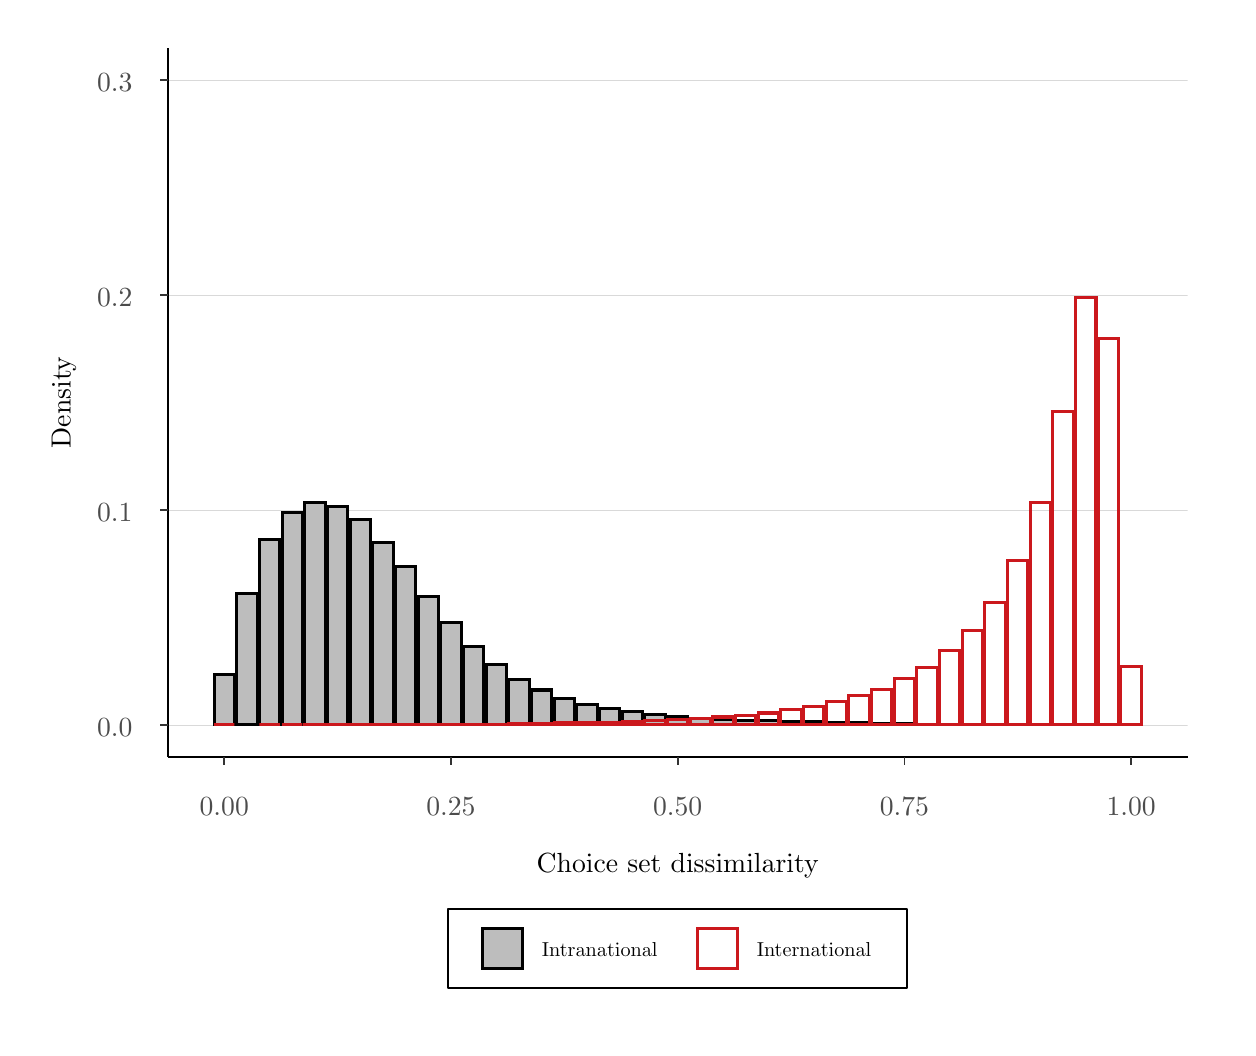
\begin{tikzpicture}[x=1pt,y=1pt]
\definecolor{fillColor}{RGB}{255,255,255}
\path[use as bounding box,fill=fillColor,fill opacity=0.00] (0,0) rectangle (433.62,361.35);
\begin{scope}
\path[clip] (  0.00,  0.00) rectangle (433.62,361.35);
\definecolor{drawColor}{RGB}{255,255,255}
\definecolor{fillColor}{RGB}{255,255,255}

\path[draw=drawColor,line width= 0.6pt,line join=round,line cap=round,fill=fillColor] (  0.00,  0.00) rectangle (433.62,361.35);
\end{scope}
\begin{scope}
\path[clip] ( 50.59, 97.75) rectangle (419.17,354.12);
\definecolor{drawColor}{RGB}{255,255,255}

\path[draw=drawColor,line width= 0.3pt,line join=round] ( 50.59,148.25) --
	(419.17,148.25);

\path[draw=drawColor,line width= 0.3pt,line join=round] ( 50.59,225.94) --
	(419.17,225.94);

\path[draw=drawColor,line width= 0.3pt,line join=round] ( 50.59,303.62) --
	(419.17,303.62);

\path[draw=drawColor,line width= 0.3pt,line join=round] (111.99, 97.75) --
	(111.99,354.12);

\path[draw=drawColor,line width= 0.3pt,line join=round] (193.92, 97.75) --
	(193.92,354.12);

\path[draw=drawColor,line width= 0.3pt,line join=round] (275.84, 97.75) --
	(275.84,354.12);

\path[draw=drawColor,line width= 0.3pt,line join=round] (357.76, 97.75) --
	(357.76,354.12);
\definecolor{drawColor}{gray}{0.85}

\path[draw=drawColor,line width= 0.1pt,line join=round] ( 50.59,109.40) --
	(419.17,109.40);

\path[draw=drawColor,line width= 0.1pt,line join=round] ( 50.59,187.09) --
	(419.17,187.09);

\path[draw=drawColor,line width= 0.1pt,line join=round] ( 50.59,264.78) --
	(419.17,264.78);

\path[draw=drawColor,line width= 0.1pt,line join=round] ( 50.59,342.47) --
	(419.17,342.47);
\definecolor{drawColor}{RGB}{0,0,0}
\definecolor{fillColor}{gray}{0.74}

\path[draw=drawColor,line width= 1.1pt,line cap=rect,fill=fillColor] ( 67.34,109.40) rectangle ( 74.72,127.47);
\definecolor{drawColor}{RGB}{203,24,29}

\path[draw=drawColor,line width= 1.1pt,line cap=rect] ( 67.34,109.40) rectangle ( 74.72,109.40);
\definecolor{drawColor}{RGB}{0,0,0}

\path[draw=drawColor,line width= 1.1pt,line cap=rect,fill=fillColor] ( 75.54,109.40) rectangle ( 82.91,156.97);

\path[draw=drawColor,line width= 1.1pt,line cap=rect,fill=fillColor] ( 83.73,109.40) rectangle ( 91.10,176.40);
\definecolor{drawColor}{RGB}{203,24,29}

\path[draw=drawColor,line width= 1.1pt,line cap=rect] ( 83.73,109.40) rectangle ( 91.10,109.40);
\definecolor{drawColor}{RGB}{0,0,0}

\path[draw=drawColor,line width= 1.1pt,line cap=rect,fill=fillColor] ( 91.92,109.40) rectangle ( 99.29,186.05);
\definecolor{drawColor}{RGB}{203,24,29}

\path[draw=drawColor,line width= 1.1pt,line cap=rect] ( 91.92,109.40) rectangle ( 99.29,109.40);
\definecolor{drawColor}{RGB}{0,0,0}

\path[draw=drawColor,line width= 1.1pt,line cap=rect,fill=fillColor] (100.11,109.40) rectangle (107.49,189.91);
\definecolor{drawColor}{RGB}{203,24,29}

\path[draw=drawColor,line width= 1.1pt,line cap=rect] (100.11,109.40) rectangle (107.49,109.41);
\definecolor{drawColor}{RGB}{0,0,0}

\path[draw=drawColor,line width= 1.1pt,line cap=rect,fill=fillColor] (108.31,109.40) rectangle (115.68,188.45);
\definecolor{drawColor}{RGB}{203,24,29}

\path[draw=drawColor,line width= 1.1pt,line cap=rect] (108.31,109.40) rectangle (115.68,109.41);
\definecolor{drawColor}{RGB}{0,0,0}

\path[draw=drawColor,line width= 1.1pt,line cap=rect,fill=fillColor] (116.50,109.40) rectangle (123.87,183.53);
\definecolor{drawColor}{RGB}{203,24,29}

\path[draw=drawColor,line width= 1.1pt,line cap=rect] (116.50,109.40) rectangle (123.87,109.42);
\definecolor{drawColor}{RGB}{0,0,0}

\path[draw=drawColor,line width= 1.1pt,line cap=rect,fill=fillColor] (124.69,109.40) rectangle (132.06,175.16);
\definecolor{drawColor}{RGB}{203,24,29}

\path[draw=drawColor,line width= 1.1pt,line cap=rect] (124.69,109.40) rectangle (132.06,109.44);
\definecolor{drawColor}{RGB}{0,0,0}

\path[draw=drawColor,line width= 1.1pt,line cap=rect,fill=fillColor] (132.88,109.40) rectangle (140.26,166.57);
\definecolor{drawColor}{RGB}{203,24,29}

\path[draw=drawColor,line width= 1.1pt,line cap=rect] (132.88,109.40) rectangle (140.26,109.46);
\definecolor{drawColor}{RGB}{0,0,0}

\path[draw=drawColor,line width= 1.1pt,line cap=rect,fill=fillColor] (141.08,109.40) rectangle (148.45,155.83);
\definecolor{drawColor}{RGB}{203,24,29}

\path[draw=drawColor,line width= 1.1pt,line cap=rect] (141.08,109.40) rectangle (148.45,109.48);
\definecolor{drawColor}{RGB}{0,0,0}

\path[draw=drawColor,line width= 1.1pt,line cap=rect,fill=fillColor] (149.27,109.40) rectangle (156.64,146.52);
\definecolor{drawColor}{RGB}{203,24,29}

\path[draw=drawColor,line width= 1.1pt,line cap=rect] (149.27,109.40) rectangle (156.64,109.54);
\definecolor{drawColor}{RGB}{0,0,0}

\path[draw=drawColor,line width= 1.1pt,line cap=rect,fill=fillColor] (157.46,109.40) rectangle (164.83,137.75);
\definecolor{drawColor}{RGB}{203,24,29}

\path[draw=drawColor,line width= 1.1pt,line cap=rect] (157.46,109.40) rectangle (164.83,109.57);
\definecolor{drawColor}{RGB}{0,0,0}

\path[draw=drawColor,line width= 1.1pt,line cap=rect,fill=fillColor] (165.65,109.40) rectangle (173.03,131.25);
\definecolor{drawColor}{RGB}{203,24,29}

\path[draw=drawColor,line width= 1.1pt,line cap=rect] (165.65,109.40) rectangle (173.03,109.68);
\definecolor{drawColor}{RGB}{0,0,0}

\path[draw=drawColor,line width= 1.1pt,line cap=rect,fill=fillColor] (173.85,109.40) rectangle (181.22,125.94);
\definecolor{drawColor}{RGB}{203,24,29}

\path[draw=drawColor,line width= 1.1pt,line cap=rect] (173.85,109.40) rectangle (181.22,109.79);
\definecolor{drawColor}{RGB}{0,0,0}

\path[draw=drawColor,line width= 1.1pt,line cap=rect,fill=fillColor] (182.04,109.40) rectangle (189.41,122.01);
\definecolor{drawColor}{RGB}{203,24,29}

\path[draw=drawColor,line width= 1.1pt,line cap=rect] (182.04,109.40) rectangle (189.41,109.89);
\definecolor{drawColor}{RGB}{0,0,0}

\path[draw=drawColor,line width= 1.1pt,line cap=rect,fill=fillColor] (190.23,109.40) rectangle (197.60,119.09);
\definecolor{drawColor}{RGB}{203,24,29}

\path[draw=drawColor,line width= 1.1pt,line cap=rect] (190.23,109.40) rectangle (197.60,110.09);
\definecolor{drawColor}{RGB}{0,0,0}

\path[draw=drawColor,line width= 1.1pt,line cap=rect,fill=fillColor] (198.42,109.40) rectangle (205.80,116.93);
\definecolor{drawColor}{RGB}{203,24,29}

\path[draw=drawColor,line width= 1.1pt,line cap=rect] (198.42,109.40) rectangle (205.80,110.26);
\definecolor{drawColor}{RGB}{0,0,0}

\path[draw=drawColor,line width= 1.1pt,line cap=rect,fill=fillColor] (206.61,109.40) rectangle (213.99,115.28);
\definecolor{drawColor}{RGB}{203,24,29}

\path[draw=drawColor,line width= 1.1pt,line cap=rect] (206.61,109.40) rectangle (213.99,110.43);
\definecolor{drawColor}{RGB}{0,0,0}

\path[draw=drawColor,line width= 1.1pt,line cap=rect,fill=fillColor] (214.81,109.40) rectangle (222.18,114.17);
\definecolor{drawColor}{RGB}{203,24,29}

\path[draw=drawColor,line width= 1.1pt,line cap=rect] (214.81,109.40) rectangle (222.18,110.72);
\definecolor{drawColor}{RGB}{0,0,0}

\path[draw=drawColor,line width= 1.1pt,line cap=rect,fill=fillColor] (223.00,109.40) rectangle (230.37,113.05);
\definecolor{drawColor}{RGB}{203,24,29}

\path[draw=drawColor,line width= 1.1pt,line cap=rect] (223.00,109.40) rectangle (230.37,110.89);
\definecolor{drawColor}{RGB}{0,0,0}

\path[draw=drawColor,line width= 1.1pt,line cap=rect,fill=fillColor] (231.19,109.40) rectangle (238.56,112.50);
\definecolor{drawColor}{RGB}{203,24,29}

\path[draw=drawColor,line width= 1.1pt,line cap=rect] (231.19,109.40) rectangle (238.56,111.42);
\definecolor{drawColor}{RGB}{0,0,0}

\path[draw=drawColor,line width= 1.1pt,line cap=rect,fill=fillColor] (239.38,109.40) rectangle (246.76,111.86);
\definecolor{drawColor}{RGB}{203,24,29}

\path[draw=drawColor,line width= 1.1pt,line cap=rect] (239.38,109.40) rectangle (246.76,111.74);
\definecolor{drawColor}{RGB}{0,0,0}

\path[draw=drawColor,line width= 1.1pt,line cap=rect,fill=fillColor] (247.58,109.40) rectangle (254.95,111.40);
\definecolor{drawColor}{RGB}{203,24,29}

\path[draw=drawColor,line width= 1.1pt,line cap=rect] (247.58,109.40) rectangle (254.95,112.26);
\definecolor{drawColor}{RGB}{0,0,0}

\path[draw=drawColor,line width= 1.1pt,line cap=rect,fill=fillColor] (255.77,109.40) rectangle (263.14,111.13);
\definecolor{drawColor}{RGB}{203,24,29}

\path[draw=drawColor,line width= 1.1pt,line cap=rect] (255.77,109.40) rectangle (263.14,112.80);
\definecolor{drawColor}{RGB}{0,0,0}

\path[draw=drawColor,line width= 1.1pt,line cap=rect,fill=fillColor] (263.96,109.40) rectangle (271.33,110.95);
\definecolor{drawColor}{RGB}{203,24,29}

\path[draw=drawColor,line width= 1.1pt,line cap=rect] (263.96,109.40) rectangle (271.33,113.71);
\definecolor{drawColor}{RGB}{0,0,0}

\path[draw=drawColor,line width= 1.1pt,line cap=rect,fill=fillColor] (272.15,109.40) rectangle (279.53,110.72);
\definecolor{drawColor}{RGB}{203,24,29}

\path[draw=drawColor,line width= 1.1pt,line cap=rect] (272.15,109.40) rectangle (279.53,114.84);
\definecolor{drawColor}{RGB}{0,0,0}

\path[draw=drawColor,line width= 1.1pt,line cap=rect,fill=fillColor] (280.35,109.40) rectangle (287.72,110.46);
\definecolor{drawColor}{RGB}{203,24,29}

\path[draw=drawColor,line width= 1.1pt,line cap=rect] (280.35,109.40) rectangle (287.72,116.03);
\definecolor{drawColor}{RGB}{0,0,0}

\path[draw=drawColor,line width= 1.1pt,line cap=rect,fill=fillColor] (288.54,109.40) rectangle (295.91,110.33);
\definecolor{drawColor}{RGB}{203,24,29}

\path[draw=drawColor,line width= 1.1pt,line cap=rect] (288.54,109.40) rectangle (295.91,117.94);
\definecolor{drawColor}{RGB}{0,0,0}

\path[draw=drawColor,line width= 1.1pt,line cap=rect,fill=fillColor] (296.73,109.40) rectangle (304.10,110.13);
\definecolor{drawColor}{RGB}{203,24,29}

\path[draw=drawColor,line width= 1.1pt,line cap=rect] (296.73,109.40) rectangle (304.10,119.87);
\definecolor{drawColor}{RGB}{0,0,0}

\path[draw=drawColor,line width= 1.1pt,line cap=rect,fill=fillColor] (304.92,109.40) rectangle (312.30,109.99);
\definecolor{drawColor}{RGB}{203,24,29}

\path[draw=drawColor,line width= 1.1pt,line cap=rect] (304.92,109.40) rectangle (312.30,122.25);
\definecolor{drawColor}{RGB}{0,0,0}

\path[draw=drawColor,line width= 1.1pt,line cap=rect,fill=fillColor] (313.12,109.40) rectangle (320.49,109.85);
\definecolor{drawColor}{RGB}{203,24,29}

\path[draw=drawColor,line width= 1.1pt,line cap=rect] (313.12,109.40) rectangle (320.49,126.29);
\definecolor{drawColor}{RGB}{0,0,0}

\path[draw=drawColor,line width= 1.1pt,line cap=rect,fill=fillColor] (321.31,109.40) rectangle (328.68,109.66);
\definecolor{drawColor}{RGB}{203,24,29}

\path[draw=drawColor,line width= 1.1pt,line cap=rect] (321.31,109.40) rectangle (328.68,130.20);
\definecolor{drawColor}{RGB}{0,0,0}

\path[draw=drawColor,line width= 1.1pt,line cap=rect,fill=fillColor] (329.50,109.40) rectangle (336.87,109.58);
\definecolor{drawColor}{RGB}{203,24,29}

\path[draw=drawColor,line width= 1.1pt,line cap=rect] (329.50,109.40) rectangle (336.87,136.34);
\definecolor{drawColor}{RGB}{0,0,0}

\path[draw=drawColor,line width= 1.1pt,line cap=rect,fill=fillColor] (337.69,109.40) rectangle (345.07,109.51);
\definecolor{drawColor}{RGB}{203,24,29}

\path[draw=drawColor,line width= 1.1pt,line cap=rect] (337.69,109.40) rectangle (345.07,143.53);
\definecolor{drawColor}{RGB}{0,0,0}

\path[draw=drawColor,line width= 1.1pt,line cap=rect,fill=fillColor] (345.89,109.40) rectangle (353.26,109.48);
\definecolor{drawColor}{RGB}{203,24,29}

\path[draw=drawColor,line width= 1.1pt,line cap=rect] (345.89,109.40) rectangle (353.26,153.78);
\definecolor{drawColor}{RGB}{0,0,0}

\path[draw=drawColor,line width= 1.1pt,line cap=rect,fill=fillColor] (354.08,109.40) rectangle (361.45,109.47);
\definecolor{drawColor}{RGB}{203,24,29}

\path[draw=drawColor,line width= 1.1pt,line cap=rect] (354.08,109.40) rectangle (361.45,168.82);
\definecolor{drawColor}{RGB}{0,0,0}

\path[draw=drawColor,line width= 1.1pt,line cap=rect,fill=fillColor] (362.27,109.40) rectangle (369.64,109.43);
\definecolor{drawColor}{RGB}{203,24,29}

\path[draw=drawColor,line width= 1.1pt,line cap=rect] (362.27,109.40) rectangle (369.64,189.68);
\definecolor{drawColor}{RGB}{0,0,0}

\path[draw=drawColor,line width= 1.1pt,line cap=rect,fill=fillColor] (370.46,109.40) rectangle (377.84,109.41);
\definecolor{drawColor}{RGB}{203,24,29}

\path[draw=drawColor,line width= 1.1pt,line cap=rect] (370.46,109.40) rectangle (377.84,222.73);

\path[draw=drawColor,line width= 1.1pt,line cap=rect] (378.65,109.40) rectangle (386.03,263.73);

\path[draw=drawColor,line width= 1.1pt,line cap=rect] (386.85,109.40) rectangle (394.22,248.93);

\path[draw=drawColor,line width= 1.1pt,line cap=rect] (395.04,109.40) rectangle (402.41,130.40);
\end{scope}
\begin{scope}
\path[clip] (  0.00,  0.00) rectangle (433.62,361.35);
\definecolor{drawColor}{RGB}{0,0,0}

\path[draw=drawColor,line width= 0.6pt,line join=round] ( 50.59, 97.75) --
	( 50.59,354.12);
\end{scope}
\begin{scope}
\path[clip] (  0.00,  0.00) rectangle (433.62,361.35);
\definecolor{drawColor}{gray}{0.30}

\node[text=drawColor,anchor=base east,inner sep=0pt, outer sep=0pt, scale=  1.00] at ( 37.84,105.27) {0.0};

\node[text=drawColor,anchor=base east,inner sep=0pt, outer sep=0pt, scale=  1.00] at ( 37.84,182.96) {0.1};

\node[text=drawColor,anchor=base east,inner sep=0pt, outer sep=0pt, scale=  1.00] at ( 37.84,260.65) {0.2};

\node[text=drawColor,anchor=base east,inner sep=0pt, outer sep=0pt, scale=  1.00] at ( 37.84,338.34) {0.3};
\end{scope}
\begin{scope}
\path[clip] (  0.00,  0.00) rectangle (433.62,361.35);
\definecolor{drawColor}{gray}{0.20}

\path[draw=drawColor,line width= 0.6pt,line join=round] ( 47.84,109.40) --
	( 50.59,109.40);

\path[draw=drawColor,line width= 0.6pt,line join=round] ( 47.84,187.09) --
	( 50.59,187.09);

\path[draw=drawColor,line width= 0.6pt,line join=round] ( 47.84,264.78) --
	( 50.59,264.78);

\path[draw=drawColor,line width= 0.6pt,line join=round] ( 47.84,342.47) --
	( 50.59,342.47);
\end{scope}
\begin{scope}
\path[clip] (  0.00,  0.00) rectangle (433.62,361.35);
\definecolor{drawColor}{RGB}{0,0,0}

\path[draw=drawColor,line width= 0.6pt,line join=round] ( 50.59, 97.75) --
	(419.17, 97.75);
\end{scope}
\begin{scope}
\path[clip] (  0.00,  0.00) rectangle (433.62,361.35);
\definecolor{drawColor}{gray}{0.20}

\path[draw=drawColor,line width= 0.6pt,line join=round] ( 71.03, 95.00) --
	( 71.03, 97.75);

\path[draw=drawColor,line width= 0.6pt,line join=round] (152.95, 95.00) --
	(152.95, 97.75);

\path[draw=drawColor,line width= 0.6pt,line join=round] (234.88, 95.00) --
	(234.88, 97.75);

\path[draw=drawColor,line width= 0.6pt,line join=round] (316.80, 95.00) --
	(316.80, 97.75);

\path[draw=drawColor,line width= 0.6pt,line join=round] (398.73, 95.00) --
	(398.73, 97.75);
\end{scope}
\begin{scope}
\path[clip] (  0.00,  0.00) rectangle (433.62,361.35);
\definecolor{drawColor}{gray}{0.30}

\node[text=drawColor,anchor=base,inner sep=0pt, outer sep=0pt, scale=  1.00] at ( 71.03, 76.73) {0.00};

\node[text=drawColor,anchor=base,inner sep=0pt, outer sep=0pt, scale=  1.00] at (152.95, 76.73) {0.25};

\node[text=drawColor,anchor=base,inner sep=0pt, outer sep=0pt, scale=  1.00] at (234.88, 76.73) {0.50};

\node[text=drawColor,anchor=base,inner sep=0pt, outer sep=0pt, scale=  1.00] at (316.80, 76.73) {0.75};

\node[text=drawColor,anchor=base,inner sep=0pt, outer sep=0pt, scale=  1.00] at (398.73, 76.73) {1.00};
\end{scope}
\begin{scope}
\path[clip] (  0.00,  0.00) rectangle (433.62,361.35);
\definecolor{drawColor}{RGB}{0,0,0}

\node[text=drawColor,anchor=base,inner sep=0pt, outer sep=0pt, scale=  1.00] at (234.88, 56.13) {Choice set dissimilarity};
\end{scope}
\begin{scope}
\path[clip] (  0.00,  0.00) rectangle (433.62,361.35);
\definecolor{drawColor}{RGB}{0,0,0}

\node[text=drawColor,rotate= 90.00,anchor=base,inner sep=0pt, outer sep=0pt, scale=  1.00] at ( 15.49,225.94) {Density};
\end{scope}
\begin{scope}
\path[clip] (  0.00,  0.00) rectangle (433.62,361.35);
\definecolor{drawColor}{RGB}{0,0,0}
\definecolor{fillColor}{RGB}{255,255,255}

\path[draw=drawColor,line width= 0.6pt,line join=round,line cap=round,fill=fillColor] (151.97, 14.45) rectangle (317.79, 42.80);
\end{scope}
\begin{scope}
\path[clip] (  0.00,  0.00) rectangle (433.62,361.35);

\path[] (162.97, 19.95) rectangle (180.32, 37.30);
\end{scope}
\begin{scope}
\path[clip] (  0.00,  0.00) rectangle (433.62,361.35);
\definecolor{drawColor}{RGB}{0,0,0}
\definecolor{fillColor}{gray}{0.74}

\path[draw=drawColor,line width= 1.1pt,line cap=rect,fill=fillColor] (164.39, 21.38) rectangle (178.89, 35.88);
\end{scope}
\begin{scope}
\path[clip] (  0.00,  0.00) rectangle (433.62,361.35);

\path[] (240.62, 19.95) rectangle (257.96, 37.30);
\end{scope}
\begin{scope}
\path[clip] (  0.00,  0.00) rectangle (433.62,361.35);
\definecolor{drawColor}{RGB}{203,24,29}

\path[draw=drawColor,line width= 1.1pt,line cap=rect] (242.04, 21.38) rectangle (256.54, 35.88);
\end{scope}
\begin{scope}
\path[clip] (  0.00,  0.00) rectangle (433.62,361.35);
\definecolor{drawColor}{RGB}{0,0,0}

\node[text=drawColor,anchor=base west,inner sep=0pt, outer sep=0pt, scale=  0.73] at (185.82, 25.60) {Intranational};
\end{scope}
\begin{scope}
\path[clip] (  0.00,  0.00) rectangle (433.62,361.35);
\definecolor{drawColor}{RGB}{0,0,0}

\node[text=drawColor,anchor=base west,inner sep=0pt, outer sep=0pt, scale=  0.73] at (263.46, 25.60) {International};
\end{scope}
\end{tikzpicture}
}
     \end{subfigure}
     \begin{subfigure}[t]{.49\textwidth}
         \centering
         \caption{$\lambda^{B,ll'}_{p,t}$}
         \label{fig: redform_bar_e}
         \scalebox{0.45}{% Created by tikzDevice version 0.12.3.1 on 2022-10-03 21:44:12
% !TEX encoding = UTF-8 Unicode
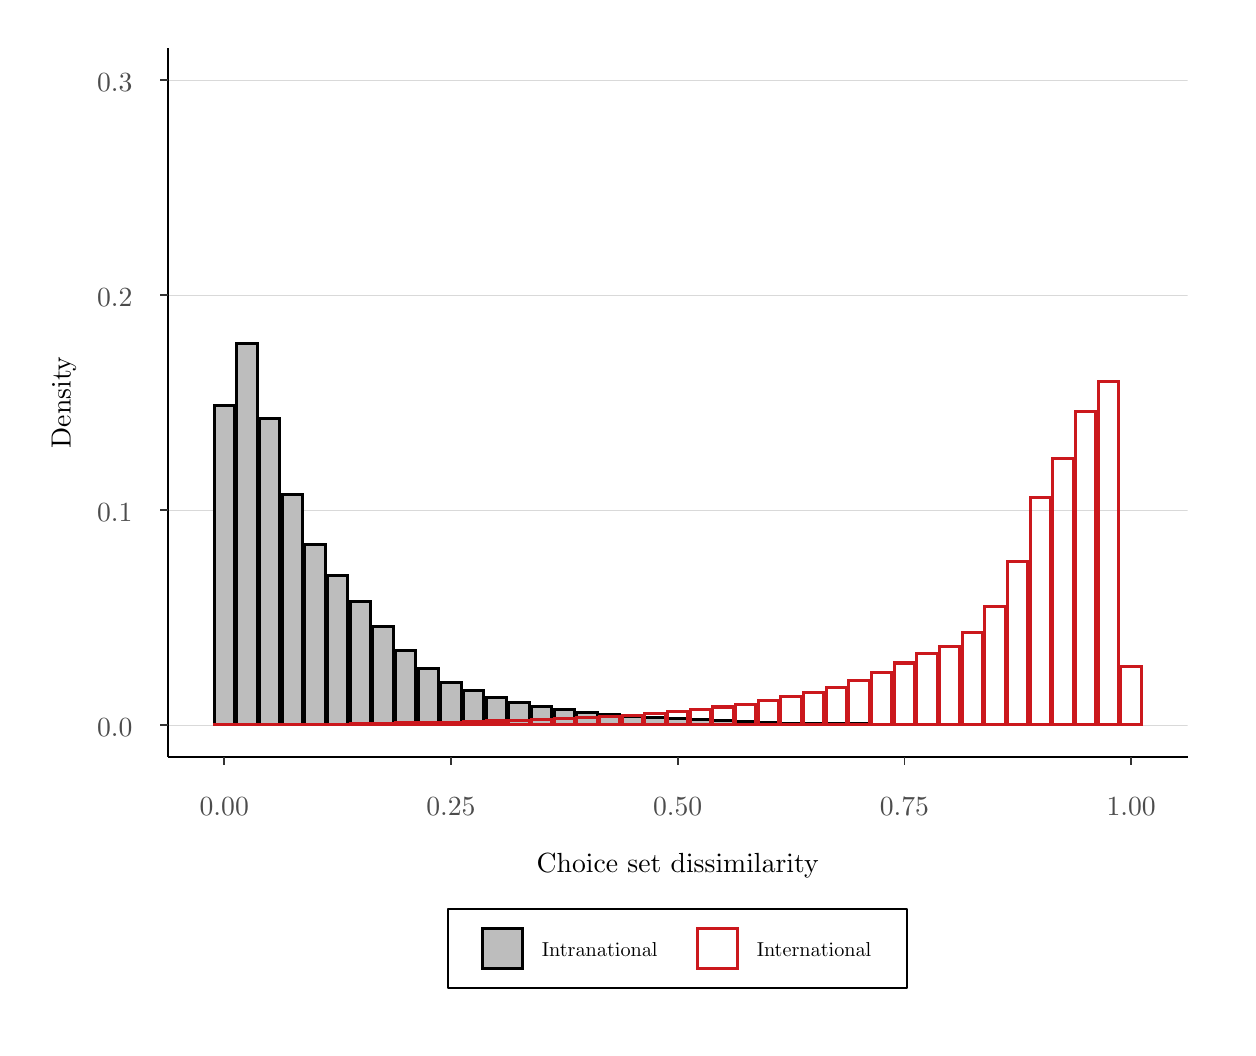
\begin{tikzpicture}[x=1pt,y=1pt]
\definecolor{fillColor}{RGB}{255,255,255}
\path[use as bounding box,fill=fillColor,fill opacity=0.00] (0,0) rectangle (433.62,361.35);
\begin{scope}
\path[clip] (  0.00,  0.00) rectangle (433.62,361.35);
\definecolor{drawColor}{RGB}{255,255,255}
\definecolor{fillColor}{RGB}{255,255,255}

\path[draw=drawColor,line width= 0.6pt,line join=round,line cap=round,fill=fillColor] (  0.00,  0.00) rectangle (433.62,361.35);
\end{scope}
\begin{scope}
\path[clip] ( 50.59, 97.75) rectangle (419.17,354.12);
\definecolor{drawColor}{RGB}{255,255,255}

\path[draw=drawColor,line width= 0.3pt,line join=round] ( 50.59,148.25) --
	(419.17,148.25);

\path[draw=drawColor,line width= 0.3pt,line join=round] ( 50.59,225.94) --
	(419.17,225.94);

\path[draw=drawColor,line width= 0.3pt,line join=round] ( 50.59,303.62) --
	(419.17,303.62);

\path[draw=drawColor,line width= 0.3pt,line join=round] (111.99, 97.75) --
	(111.99,354.12);

\path[draw=drawColor,line width= 0.3pt,line join=round] (193.92, 97.75) --
	(193.92,354.12);

\path[draw=drawColor,line width= 0.3pt,line join=round] (275.84, 97.75) --
	(275.84,354.12);

\path[draw=drawColor,line width= 0.3pt,line join=round] (357.76, 97.75) --
	(357.76,354.12);
\definecolor{drawColor}{gray}{0.85}

\path[draw=drawColor,line width= 0.1pt,line join=round] ( 50.59,109.40) --
	(419.17,109.40);

\path[draw=drawColor,line width= 0.1pt,line join=round] ( 50.59,187.09) --
	(419.17,187.09);

\path[draw=drawColor,line width= 0.1pt,line join=round] ( 50.59,264.78) --
	(419.17,264.78);

\path[draw=drawColor,line width= 0.1pt,line join=round] ( 50.59,342.47) --
	(419.17,342.47);
\definecolor{drawColor}{RGB}{0,0,0}
\definecolor{fillColor}{gray}{0.74}

\path[draw=drawColor,line width= 1.1pt,line cap=rect,fill=fillColor] ( 67.34,109.40) rectangle ( 74.72,224.75);
\definecolor{drawColor}{RGB}{203,24,29}

\path[draw=drawColor,line width= 1.1pt,line cap=rect] ( 67.34,109.40) rectangle ( 74.72,109.41);
\definecolor{drawColor}{RGB}{0,0,0}

\path[draw=drawColor,line width= 1.1pt,line cap=rect,fill=fillColor] ( 75.54,109.40) rectangle ( 82.91,247.28);
\definecolor{drawColor}{RGB}{203,24,29}

\path[draw=drawColor,line width= 1.1pt,line cap=rect] ( 75.54,109.40) rectangle ( 82.91,109.48);
\definecolor{drawColor}{RGB}{0,0,0}

\path[draw=drawColor,line width= 1.1pt,line cap=rect,fill=fillColor] ( 83.73,109.40) rectangle ( 91.10,220.14);
\definecolor{drawColor}{RGB}{203,24,29}

\path[draw=drawColor,line width= 1.1pt,line cap=rect] ( 83.73,109.40) rectangle ( 91.10,109.52);
\definecolor{drawColor}{RGB}{0,0,0}

\path[draw=drawColor,line width= 1.1pt,line cap=rect,fill=fillColor] ( 91.92,109.40) rectangle ( 99.29,192.63);
\definecolor{drawColor}{RGB}{203,24,29}

\path[draw=drawColor,line width= 1.1pt,line cap=rect] ( 91.92,109.40) rectangle ( 99.29,109.58);
\definecolor{drawColor}{RGB}{0,0,0}

\path[draw=drawColor,line width= 1.1pt,line cap=rect,fill=fillColor] (100.11,109.40) rectangle (107.49,174.64);
\definecolor{drawColor}{RGB}{203,24,29}

\path[draw=drawColor,line width= 1.1pt,line cap=rect] (100.11,109.40) rectangle (107.49,109.63);
\definecolor{drawColor}{RGB}{0,0,0}

\path[draw=drawColor,line width= 1.1pt,line cap=rect,fill=fillColor] (108.31,109.40) rectangle (115.68,163.34);
\definecolor{drawColor}{RGB}{203,24,29}

\path[draw=drawColor,line width= 1.1pt,line cap=rect] (108.31,109.40) rectangle (115.68,109.71);
\definecolor{drawColor}{RGB}{0,0,0}

\path[draw=drawColor,line width= 1.1pt,line cap=rect,fill=fillColor] (116.50,109.40) rectangle (123.87,153.97);
\definecolor{drawColor}{RGB}{203,24,29}

\path[draw=drawColor,line width= 1.1pt,line cap=rect] (116.50,109.40) rectangle (123.87,109.83);
\definecolor{drawColor}{RGB}{0,0,0}

\path[draw=drawColor,line width= 1.1pt,line cap=rect,fill=fillColor] (124.69,109.40) rectangle (132.06,144.86);
\definecolor{drawColor}{RGB}{203,24,29}

\path[draw=drawColor,line width= 1.1pt,line cap=rect] (124.69,109.40) rectangle (132.06,109.92);
\definecolor{drawColor}{RGB}{0,0,0}

\path[draw=drawColor,line width= 1.1pt,line cap=rect,fill=fillColor] (132.88,109.40) rectangle (140.26,136.40);
\definecolor{drawColor}{RGB}{203,24,29}

\path[draw=drawColor,line width= 1.1pt,line cap=rect] (132.88,109.40) rectangle (140.26,110.09);
\definecolor{drawColor}{RGB}{0,0,0}

\path[draw=drawColor,line width= 1.1pt,line cap=rect,fill=fillColor] (141.08,109.40) rectangle (148.45,129.74);
\definecolor{drawColor}{RGB}{203,24,29}

\path[draw=drawColor,line width= 1.1pt,line cap=rect] (141.08,109.40) rectangle (148.45,110.27);
\definecolor{drawColor}{RGB}{0,0,0}

\path[draw=drawColor,line width= 1.1pt,line cap=rect,fill=fillColor] (149.27,109.40) rectangle (156.64,124.84);
\definecolor{drawColor}{RGB}{203,24,29}

\path[draw=drawColor,line width= 1.1pt,line cap=rect] (149.27,109.40) rectangle (156.64,110.44);
\definecolor{drawColor}{RGB}{0,0,0}

\path[draw=drawColor,line width= 1.1pt,line cap=rect,fill=fillColor] (157.46,109.40) rectangle (164.83,121.85);
\definecolor{drawColor}{RGB}{203,24,29}

\path[draw=drawColor,line width= 1.1pt,line cap=rect] (157.46,109.40) rectangle (164.83,110.65);
\definecolor{drawColor}{RGB}{0,0,0}

\path[draw=drawColor,line width= 1.1pt,line cap=rect,fill=fillColor] (165.65,109.40) rectangle (173.03,119.47);
\definecolor{drawColor}{RGB}{203,24,29}

\path[draw=drawColor,line width= 1.1pt,line cap=rect] (165.65,109.40) rectangle (173.03,110.81);
\definecolor{drawColor}{RGB}{0,0,0}

\path[draw=drawColor,line width= 1.1pt,line cap=rect,fill=fillColor] (173.85,109.40) rectangle (181.22,117.54);
\definecolor{drawColor}{RGB}{203,24,29}

\path[draw=drawColor,line width= 1.1pt,line cap=rect] (173.85,109.40) rectangle (181.22,111.01);
\definecolor{drawColor}{RGB}{0,0,0}

\path[draw=drawColor,line width= 1.1pt,line cap=rect,fill=fillColor] (182.04,109.40) rectangle (189.41,116.15);
\definecolor{drawColor}{RGB}{203,24,29}

\path[draw=drawColor,line width= 1.1pt,line cap=rect] (182.04,109.40) rectangle (189.41,111.24);
\definecolor{drawColor}{RGB}{0,0,0}

\path[draw=drawColor,line width= 1.1pt,line cap=rect,fill=fillColor] (190.23,109.40) rectangle (197.60,114.95);
\definecolor{drawColor}{RGB}{203,24,29}

\path[draw=drawColor,line width= 1.1pt,line cap=rect] (190.23,109.40) rectangle (197.60,111.56);
\definecolor{drawColor}{RGB}{0,0,0}

\path[draw=drawColor,line width= 1.1pt,line cap=rect,fill=fillColor] (198.42,109.40) rectangle (205.80,113.82);
\definecolor{drawColor}{RGB}{203,24,29}

\path[draw=drawColor,line width= 1.1pt,line cap=rect] (198.42,109.40) rectangle (205.80,111.93);
\definecolor{drawColor}{RGB}{0,0,0}

\path[draw=drawColor,line width= 1.1pt,line cap=rect,fill=fillColor] (206.61,109.40) rectangle (213.99,113.03);
\definecolor{drawColor}{RGB}{203,24,29}

\path[draw=drawColor,line width= 1.1pt,line cap=rect] (206.61,109.40) rectangle (213.99,112.33);
\definecolor{drawColor}{RGB}{0,0,0}

\path[draw=drawColor,line width= 1.1pt,line cap=rect,fill=fillColor] (214.81,109.40) rectangle (222.18,112.46);
\definecolor{drawColor}{RGB}{203,24,29}

\path[draw=drawColor,line width= 1.1pt,line cap=rect] (214.81,109.40) rectangle (222.18,112.79);
\definecolor{drawColor}{RGB}{0,0,0}

\path[draw=drawColor,line width= 1.1pt,line cap=rect,fill=fillColor] (223.00,109.40) rectangle (230.37,112.09);
\definecolor{drawColor}{RGB}{203,24,29}

\path[draw=drawColor,line width= 1.1pt,line cap=rect] (223.00,109.40) rectangle (230.37,113.39);
\definecolor{drawColor}{RGB}{0,0,0}

\path[draw=drawColor,line width= 1.1pt,line cap=rect,fill=fillColor] (231.19,109.40) rectangle (238.56,111.76);
\definecolor{drawColor}{RGB}{203,24,29}

\path[draw=drawColor,line width= 1.1pt,line cap=rect] (231.19,109.40) rectangle (238.56,114.13);
\definecolor{drawColor}{RGB}{0,0,0}

\path[draw=drawColor,line width= 1.1pt,line cap=rect,fill=fillColor] (239.38,109.40) rectangle (246.76,111.45);
\definecolor{drawColor}{RGB}{203,24,29}

\path[draw=drawColor,line width= 1.1pt,line cap=rect] (239.38,109.40) rectangle (246.76,114.89);
\definecolor{drawColor}{RGB}{0,0,0}

\path[draw=drawColor,line width= 1.1pt,line cap=rect,fill=fillColor] (247.58,109.40) rectangle (254.95,111.06);
\definecolor{drawColor}{RGB}{203,24,29}

\path[draw=drawColor,line width= 1.1pt,line cap=rect] (247.58,109.40) rectangle (254.95,115.87);
\definecolor{drawColor}{RGB}{0,0,0}

\path[draw=drawColor,line width= 1.1pt,line cap=rect,fill=fillColor] (255.77,109.40) rectangle (263.14,110.71);
\definecolor{drawColor}{RGB}{203,24,29}

\path[draw=drawColor,line width= 1.1pt,line cap=rect] (255.77,109.40) rectangle (263.14,116.89);
\definecolor{drawColor}{RGB}{0,0,0}

\path[draw=drawColor,line width= 1.1pt,line cap=rect,fill=fillColor] (263.96,109.40) rectangle (271.33,110.30);
\definecolor{drawColor}{RGB}{203,24,29}

\path[draw=drawColor,line width= 1.1pt,line cap=rect] (263.96,109.40) rectangle (271.33,118.10);
\definecolor{drawColor}{RGB}{0,0,0}

\path[draw=drawColor,line width= 1.1pt,line cap=rect,fill=fillColor] (272.15,109.40) rectangle (279.53,110.02);
\definecolor{drawColor}{RGB}{203,24,29}

\path[draw=drawColor,line width= 1.1pt,line cap=rect] (272.15,109.40) rectangle (279.53,119.55);
\definecolor{drawColor}{RGB}{0,0,0}

\path[draw=drawColor,line width= 1.1pt,line cap=rect,fill=fillColor] (280.35,109.40) rectangle (287.72,109.84);
\definecolor{drawColor}{RGB}{203,24,29}

\path[draw=drawColor,line width= 1.1pt,line cap=rect] (280.35,109.40) rectangle (287.72,121.07);
\definecolor{drawColor}{RGB}{0,0,0}

\path[draw=drawColor,line width= 1.1pt,line cap=rect,fill=fillColor] (288.54,109.40) rectangle (295.91,109.77);
\definecolor{drawColor}{RGB}{203,24,29}

\path[draw=drawColor,line width= 1.1pt,line cap=rect] (288.54,109.40) rectangle (295.91,122.96);
\definecolor{drawColor}{RGB}{0,0,0}

\path[draw=drawColor,line width= 1.1pt,line cap=rect,fill=fillColor] (296.73,109.40) rectangle (304.10,109.74);
\definecolor{drawColor}{RGB}{203,24,29}

\path[draw=drawColor,line width= 1.1pt,line cap=rect] (296.73,109.40) rectangle (304.10,125.38);
\definecolor{drawColor}{RGB}{0,0,0}

\path[draw=drawColor,line width= 1.1pt,line cap=rect,fill=fillColor] (304.92,109.40) rectangle (312.30,109.67);
\definecolor{drawColor}{RGB}{203,24,29}

\path[draw=drawColor,line width= 1.1pt,line cap=rect] (304.92,109.40) rectangle (312.30,128.24);
\definecolor{drawColor}{RGB}{0,0,0}

\path[draw=drawColor,line width= 1.1pt,line cap=rect,fill=fillColor] (313.12,109.40) rectangle (320.49,109.60);
\definecolor{drawColor}{RGB}{203,24,29}

\path[draw=drawColor,line width= 1.1pt,line cap=rect] (313.12,109.40) rectangle (320.49,131.77);
\definecolor{drawColor}{RGB}{0,0,0}

\path[draw=drawColor,line width= 1.1pt,line cap=rect,fill=fillColor] (321.31,109.40) rectangle (328.68,109.53);
\definecolor{drawColor}{RGB}{203,24,29}

\path[draw=drawColor,line width= 1.1pt,line cap=rect] (321.31,109.40) rectangle (328.68,135.07);
\definecolor{drawColor}{RGB}{0,0,0}

\path[draw=drawColor,line width= 1.1pt,line cap=rect,fill=fillColor] (329.50,109.40) rectangle (336.87,109.49);
\definecolor{drawColor}{RGB}{203,24,29}

\path[draw=drawColor,line width= 1.1pt,line cap=rect] (329.50,109.40) rectangle (336.87,137.80);
\definecolor{drawColor}{RGB}{0,0,0}

\path[draw=drawColor,line width= 1.1pt,line cap=rect,fill=fillColor] (337.69,109.40) rectangle (345.07,109.47);
\definecolor{drawColor}{RGB}{203,24,29}

\path[draw=drawColor,line width= 1.1pt,line cap=rect] (337.69,109.40) rectangle (345.07,142.70);
\definecolor{drawColor}{RGB}{0,0,0}

\path[draw=drawColor,line width= 1.1pt,line cap=rect,fill=fillColor] (345.89,109.40) rectangle (353.26,109.49);
\definecolor{drawColor}{RGB}{203,24,29}

\path[draw=drawColor,line width= 1.1pt,line cap=rect] (345.89,109.40) rectangle (353.26,152.13);
\definecolor{drawColor}{RGB}{0,0,0}

\path[draw=drawColor,line width= 1.1pt,line cap=rect,fill=fillColor] (354.08,109.40) rectangle (361.45,109.47);
\definecolor{drawColor}{RGB}{203,24,29}

\path[draw=drawColor,line width= 1.1pt,line cap=rect] (354.08,109.40) rectangle (361.45,168.54);
\definecolor{drawColor}{RGB}{0,0,0}

\path[draw=drawColor,line width= 1.1pt,line cap=rect,fill=fillColor] (362.27,109.40) rectangle (369.64,109.44);
\definecolor{drawColor}{RGB}{203,24,29}

\path[draw=drawColor,line width= 1.1pt,line cap=rect] (362.27,109.40) rectangle (369.64,191.48);
\definecolor{drawColor}{RGB}{0,0,0}

\path[draw=drawColor,line width= 1.1pt,line cap=rect,fill=fillColor] (370.46,109.40) rectangle (377.84,109.42);
\definecolor{drawColor}{RGB}{203,24,29}

\path[draw=drawColor,line width= 1.1pt,line cap=rect] (370.46,109.40) rectangle (377.84,205.67);
\definecolor{drawColor}{RGB}{0,0,0}

\path[draw=drawColor,line width= 1.1pt,line cap=rect,fill=fillColor] (378.65,109.40) rectangle (386.03,109.41);
\definecolor{drawColor}{RGB}{203,24,29}

\path[draw=drawColor,line width= 1.1pt,line cap=rect] (378.65,109.40) rectangle (386.03,222.62);

\path[draw=drawColor,line width= 1.1pt,line cap=rect] (386.85,109.40) rectangle (394.22,233.49);

\path[draw=drawColor,line width= 1.1pt,line cap=rect] (395.04,109.40) rectangle (402.41,130.40);
\end{scope}
\begin{scope}
\path[clip] (  0.00,  0.00) rectangle (433.62,361.35);
\definecolor{drawColor}{RGB}{0,0,0}

\path[draw=drawColor,line width= 0.6pt,line join=round] ( 50.59, 97.75) --
	( 50.59,354.12);
\end{scope}
\begin{scope}
\path[clip] (  0.00,  0.00) rectangle (433.62,361.35);
\definecolor{drawColor}{gray}{0.30}

\node[text=drawColor,anchor=base east,inner sep=0pt, outer sep=0pt, scale=  1.00] at ( 37.84,105.27) {0.0};

\node[text=drawColor,anchor=base east,inner sep=0pt, outer sep=0pt, scale=  1.00] at ( 37.84,182.96) {0.1};

\node[text=drawColor,anchor=base east,inner sep=0pt, outer sep=0pt, scale=  1.00] at ( 37.84,260.65) {0.2};

\node[text=drawColor,anchor=base east,inner sep=0pt, outer sep=0pt, scale=  1.00] at ( 37.84,338.34) {0.3};
\end{scope}
\begin{scope}
\path[clip] (  0.00,  0.00) rectangle (433.62,361.35);
\definecolor{drawColor}{gray}{0.20}

\path[draw=drawColor,line width= 0.6pt,line join=round] ( 47.84,109.40) --
	( 50.59,109.40);

\path[draw=drawColor,line width= 0.6pt,line join=round] ( 47.84,187.09) --
	( 50.59,187.09);

\path[draw=drawColor,line width= 0.6pt,line join=round] ( 47.84,264.78) --
	( 50.59,264.78);

\path[draw=drawColor,line width= 0.6pt,line join=round] ( 47.84,342.47) --
	( 50.59,342.47);
\end{scope}
\begin{scope}
\path[clip] (  0.00,  0.00) rectangle (433.62,361.35);
\definecolor{drawColor}{RGB}{0,0,0}

\path[draw=drawColor,line width= 0.6pt,line join=round] ( 50.59, 97.75) --
	(419.17, 97.75);
\end{scope}
\begin{scope}
\path[clip] (  0.00,  0.00) rectangle (433.62,361.35);
\definecolor{drawColor}{gray}{0.20}

\path[draw=drawColor,line width= 0.6pt,line join=round] ( 71.03, 95.00) --
	( 71.03, 97.75);

\path[draw=drawColor,line width= 0.6pt,line join=round] (152.95, 95.00) --
	(152.95, 97.75);

\path[draw=drawColor,line width= 0.6pt,line join=round] (234.88, 95.00) --
	(234.88, 97.75);

\path[draw=drawColor,line width= 0.6pt,line join=round] (316.80, 95.00) --
	(316.80, 97.75);

\path[draw=drawColor,line width= 0.6pt,line join=round] (398.73, 95.00) --
	(398.73, 97.75);
\end{scope}
\begin{scope}
\path[clip] (  0.00,  0.00) rectangle (433.62,361.35);
\definecolor{drawColor}{gray}{0.30}

\node[text=drawColor,anchor=base,inner sep=0pt, outer sep=0pt, scale=  1.00] at ( 71.03, 76.73) {0.00};

\node[text=drawColor,anchor=base,inner sep=0pt, outer sep=0pt, scale=  1.00] at (152.95, 76.73) {0.25};

\node[text=drawColor,anchor=base,inner sep=0pt, outer sep=0pt, scale=  1.00] at (234.88, 76.73) {0.50};

\node[text=drawColor,anchor=base,inner sep=0pt, outer sep=0pt, scale=  1.00] at (316.80, 76.73) {0.75};

\node[text=drawColor,anchor=base,inner sep=0pt, outer sep=0pt, scale=  1.00] at (398.73, 76.73) {1.00};
\end{scope}
\begin{scope}
\path[clip] (  0.00,  0.00) rectangle (433.62,361.35);
\definecolor{drawColor}{RGB}{0,0,0}

\node[text=drawColor,anchor=base,inner sep=0pt, outer sep=0pt, scale=  1.00] at (234.88, 56.13) {Choice set dissimilarity};
\end{scope}
\begin{scope}
\path[clip] (  0.00,  0.00) rectangle (433.62,361.35);
\definecolor{drawColor}{RGB}{0,0,0}

\node[text=drawColor,rotate= 90.00,anchor=base,inner sep=0pt, outer sep=0pt, scale=  1.00] at ( 15.49,225.94) {Density};
\end{scope}
\begin{scope}
\path[clip] (  0.00,  0.00) rectangle (433.62,361.35);
\definecolor{drawColor}{RGB}{0,0,0}
\definecolor{fillColor}{RGB}{255,255,255}

\path[draw=drawColor,line width= 0.6pt,line join=round,line cap=round,fill=fillColor] (151.97, 14.45) rectangle (317.79, 42.80);
\end{scope}
\begin{scope}
\path[clip] (  0.00,  0.00) rectangle (433.62,361.35);

\path[] (162.97, 19.95) rectangle (180.32, 37.30);
\end{scope}
\begin{scope}
\path[clip] (  0.00,  0.00) rectangle (433.62,361.35);
\definecolor{drawColor}{RGB}{0,0,0}
\definecolor{fillColor}{gray}{0.74}

\path[draw=drawColor,line width= 1.1pt,line cap=rect,fill=fillColor] (164.39, 21.38) rectangle (178.89, 35.88);
\end{scope}
\begin{scope}
\path[clip] (  0.00,  0.00) rectangle (433.62,361.35);

\path[] (240.62, 19.95) rectangle (257.96, 37.30);
\end{scope}
\begin{scope}
\path[clip] (  0.00,  0.00) rectangle (433.62,361.35);
\definecolor{drawColor}{RGB}{203,24,29}

\path[draw=drawColor,line width= 1.1pt,line cap=rect] (242.04, 21.38) rectangle (256.54, 35.88);
\end{scope}
\begin{scope}
\path[clip] (  0.00,  0.00) rectangle (433.62,361.35);
\definecolor{drawColor}{RGB}{0,0,0}

\node[text=drawColor,anchor=base west,inner sep=0pt, outer sep=0pt, scale=  0.73] at (185.82, 25.60) {Intranational};
\end{scope}
\begin{scope}
\path[clip] (  0.00,  0.00) rectangle (433.62,361.35);
\definecolor{drawColor}{RGB}{0,0,0}

\node[text=drawColor,anchor=base west,inner sep=0pt, outer sep=0pt, scale=  0.73] at (263.46, 25.60) {International};
\end{scope}
\end{tikzpicture}
}
     \end{subfigure} \\
     \begin{subfigure}[t]{.49\textwidth}
        \centering
        \caption{$N^{F,ll'}_{p,t}$}
        \label{fig: redform_firm_c}
        \scalebox{0.45}{% Created by tikzDevice version 0.12.3.1 on 2022-10-03 21:47:02
% !TEX encoding = UTF-8 Unicode
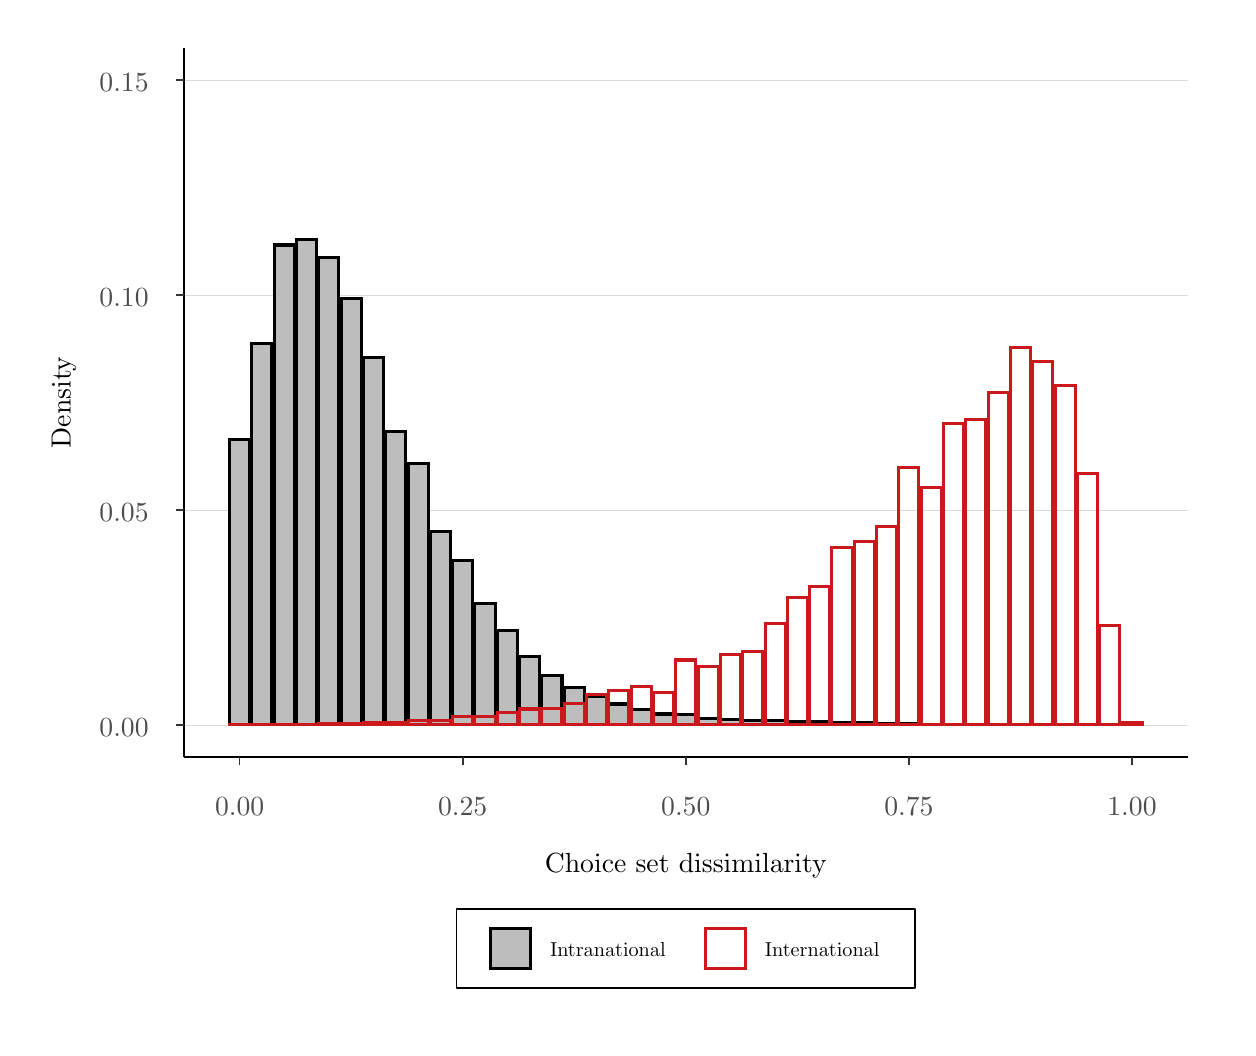
\begin{tikzpicture}[x=1pt,y=1pt]
\definecolor{fillColor}{RGB}{255,255,255}
\path[use as bounding box,fill=fillColor,fill opacity=0.00] (0,0) rectangle (433.62,361.35);
\begin{scope}
\path[clip] (  0.00,  0.00) rectangle (433.62,361.35);
\definecolor{drawColor}{RGB}{255,255,255}
\definecolor{fillColor}{RGB}{255,255,255}

\path[draw=drawColor,line width= 0.6pt,line join=round,line cap=round,fill=fillColor] ( -0.00,  0.00) rectangle (433.62,361.35);
\end{scope}
\begin{scope}
\path[clip] ( 56.47, 97.75) rectangle (419.17,354.12);
\definecolor{drawColor}{RGB}{255,255,255}

\path[draw=drawColor,line width= 0.3pt,line join=round] ( 56.47,148.25) --
	(419.17,148.25);

\path[draw=drawColor,line width= 0.3pt,line join=round] ( 56.47,225.94) --
	(419.17,225.94);

\path[draw=drawColor,line width= 0.3pt,line join=round] ( 56.47,303.62) --
	(419.17,303.62);

\path[draw=drawColor,line width= 0.3pt,line join=round] (116.89, 97.75) --
	(116.89,354.12);

\path[draw=drawColor,line width= 0.3pt,line join=round] (197.51, 97.75) --
	(197.51,354.12);

\path[draw=drawColor,line width= 0.3pt,line join=round] (278.12, 97.75) --
	(278.12,354.12);

\path[draw=drawColor,line width= 0.3pt,line join=round] (358.74, 97.75) --
	(358.74,354.12);
\definecolor{drawColor}{gray}{0.85}

\path[draw=drawColor,line width= 0.1pt,line join=round] ( 56.47,109.40) --
	(419.17,109.40);

\path[draw=drawColor,line width= 0.1pt,line join=round] ( 56.47,187.09) --
	(419.17,187.09);

\path[draw=drawColor,line width= 0.1pt,line join=round] ( 56.47,264.78) --
	(419.17,264.78);

\path[draw=drawColor,line width= 0.1pt,line join=round] ( 56.47,342.47) --
	(419.17,342.47);
\definecolor{drawColor}{RGB}{0,0,0}
\definecolor{fillColor}{gray}{0.74}

\path[draw=drawColor,line width= 1.1pt,line cap=rect,fill=fillColor] ( 72.95,109.40) rectangle ( 80.21,212.41);
\definecolor{drawColor}{RGB}{203,24,29}

\path[draw=drawColor,line width= 1.1pt,line cap=rect] ( 72.95,109.40) rectangle ( 80.21,109.61);
\definecolor{drawColor}{RGB}{0,0,0}

\path[draw=drawColor,line width= 1.1pt,line cap=rect,fill=fillColor] ( 81.01,109.40) rectangle ( 88.27,247.07);
\definecolor{drawColor}{RGB}{203,24,29}

\path[draw=drawColor,line width= 1.1pt,line cap=rect] ( 81.01,109.40) rectangle ( 88.27,109.44);
\definecolor{drawColor}{RGB}{0,0,0}

\path[draw=drawColor,line width= 1.1pt,line cap=rect,fill=fillColor] ( 89.08,109.40) rectangle ( 96.33,282.81);
\definecolor{drawColor}{RGB}{203,24,29}

\path[draw=drawColor,line width= 1.1pt,line cap=rect] ( 89.08,109.40) rectangle ( 96.33,109.49);
\definecolor{drawColor}{RGB}{0,0,0}

\path[draw=drawColor,line width= 1.1pt,line cap=rect,fill=fillColor] ( 97.14,109.40) rectangle (104.39,284.78);
\definecolor{drawColor}{RGB}{203,24,29}

\path[draw=drawColor,line width= 1.1pt,line cap=rect] ( 97.14,109.40) rectangle (104.39,109.65);
\definecolor{drawColor}{RGB}{0,0,0}

\path[draw=drawColor,line width= 1.1pt,line cap=rect,fill=fillColor] (105.20,109.40) rectangle (112.45,278.15);
\definecolor{drawColor}{RGB}{203,24,29}

\path[draw=drawColor,line width= 1.1pt,line cap=rect] (105.20,109.40) rectangle (112.45,109.75);
\definecolor{drawColor}{RGB}{0,0,0}

\path[draw=drawColor,line width= 1.1pt,line cap=rect,fill=fillColor] (113.26,109.40) rectangle (120.52,263.56);
\definecolor{drawColor}{RGB}{203,24,29}

\path[draw=drawColor,line width= 1.1pt,line cap=rect] (113.26,109.40) rectangle (120.52,109.95);
\definecolor{drawColor}{RGB}{0,0,0}

\path[draw=drawColor,line width= 1.1pt,line cap=rect,fill=fillColor] (121.32,109.40) rectangle (128.58,242.08);
\definecolor{drawColor}{RGB}{203,24,29}

\path[draw=drawColor,line width= 1.1pt,line cap=rect] (121.32,109.40) rectangle (128.58,110.14);
\definecolor{drawColor}{RGB}{0,0,0}

\path[draw=drawColor,line width= 1.1pt,line cap=rect,fill=fillColor] (129.38,109.40) rectangle (136.64,215.30);
\definecolor{drawColor}{RGB}{203,24,29}

\path[draw=drawColor,line width= 1.1pt,line cap=rect] (129.38,109.40) rectangle (136.64,110.32);
\definecolor{drawColor}{RGB}{0,0,0}

\path[draw=drawColor,line width= 1.1pt,line cap=rect,fill=fillColor] (137.45,109.40) rectangle (144.70,203.86);
\definecolor{drawColor}{RGB}{203,24,29}

\path[draw=drawColor,line width= 1.1pt,line cap=rect] (137.45,109.40) rectangle (144.70,111.14);
\definecolor{drawColor}{RGB}{0,0,0}

\path[draw=drawColor,line width= 1.1pt,line cap=rect,fill=fillColor] (145.51,109.40) rectangle (152.76,179.30);
\definecolor{drawColor}{RGB}{203,24,29}

\path[draw=drawColor,line width= 1.1pt,line cap=rect] (145.51,109.40) rectangle (152.76,110.97);
\definecolor{drawColor}{RGB}{0,0,0}

\path[draw=drawColor,line width= 1.1pt,line cap=rect,fill=fillColor] (153.57,109.40) rectangle (160.83,168.90);
\definecolor{drawColor}{RGB}{203,24,29}

\path[draw=drawColor,line width= 1.1pt,line cap=rect] (153.57,109.40) rectangle (160.83,112.55);
\definecolor{drawColor}{RGB}{0,0,0}

\path[draw=drawColor,line width= 1.1pt,line cap=rect,fill=fillColor] (161.63,109.40) rectangle (168.89,153.19);
\definecolor{drawColor}{RGB}{203,24,29}

\path[draw=drawColor,line width= 1.1pt,line cap=rect] (161.63,109.40) rectangle (168.89,112.51);
\definecolor{drawColor}{RGB}{0,0,0}

\path[draw=drawColor,line width= 1.1pt,line cap=rect,fill=fillColor] (169.69,109.40) rectangle (176.95,143.53);
\definecolor{drawColor}{RGB}{203,24,29}

\path[draw=drawColor,line width= 1.1pt,line cap=rect] (169.69,109.40) rectangle (176.95,113.98);
\definecolor{drawColor}{RGB}{0,0,0}

\path[draw=drawColor,line width= 1.1pt,line cap=rect,fill=fillColor] (177.76,109.40) rectangle (185.01,134.16);
\definecolor{drawColor}{RGB}{203,24,29}

\path[draw=drawColor,line width= 1.1pt,line cap=rect] (177.76,109.40) rectangle (185.01,115.15);
\definecolor{drawColor}{RGB}{0,0,0}

\path[draw=drawColor,line width= 1.1pt,line cap=rect,fill=fillColor] (185.82,109.40) rectangle (193.07,127.32);
\definecolor{drawColor}{RGB}{203,24,29}

\path[draw=drawColor,line width= 1.1pt,line cap=rect] (185.82,109.40) rectangle (193.07,115.32);
\definecolor{drawColor}{RGB}{0,0,0}

\path[draw=drawColor,line width= 1.1pt,line cap=rect,fill=fillColor] (193.88,109.40) rectangle (201.13,123.07);
\definecolor{drawColor}{RGB}{203,24,29}

\path[draw=drawColor,line width= 1.1pt,line cap=rect] (193.88,109.40) rectangle (201.13,117.26);
\definecolor{drawColor}{RGB}{0,0,0}

\path[draw=drawColor,line width= 1.1pt,line cap=rect,fill=fillColor] (201.94,109.40) rectangle (209.20,119.67);
\definecolor{drawColor}{RGB}{203,24,29}

\path[draw=drawColor,line width= 1.1pt,line cap=rect] (201.94,109.40) rectangle (209.20,120.43);
\definecolor{drawColor}{RGB}{0,0,0}

\path[draw=drawColor,line width= 1.1pt,line cap=rect,fill=fillColor] (210.00,109.40) rectangle (217.26,116.95);
\definecolor{drawColor}{RGB}{203,24,29}

\path[draw=drawColor,line width= 1.1pt,line cap=rect] (210.00,109.40) rectangle (217.26,121.75);
\definecolor{drawColor}{RGB}{0,0,0}

\path[draw=drawColor,line width= 1.1pt,line cap=rect,fill=fillColor] (218.06,109.40) rectangle (225.32,115.04);
\definecolor{drawColor}{RGB}{203,24,29}

\path[draw=drawColor,line width= 1.1pt,line cap=rect] (218.06,109.40) rectangle (225.32,123.14);
\definecolor{drawColor}{RGB}{0,0,0}

\path[draw=drawColor,line width= 1.1pt,line cap=rect,fill=fillColor] (226.13,109.40) rectangle (233.38,113.34);
\definecolor{drawColor}{RGB}{203,24,29}

\path[draw=drawColor,line width= 1.1pt,line cap=rect] (226.13,109.40) rectangle (233.38,121.24);
\definecolor{drawColor}{RGB}{0,0,0}

\path[draw=drawColor,line width= 1.1pt,line cap=rect,fill=fillColor] (234.19,109.40) rectangle (241.44,113.02);
\definecolor{drawColor}{RGB}{203,24,29}

\path[draw=drawColor,line width= 1.1pt,line cap=rect] (234.19,109.40) rectangle (241.44,132.86);
\definecolor{drawColor}{RGB}{0,0,0}

\path[draw=drawColor,line width= 1.1pt,line cap=rect,fill=fillColor] (242.25,109.40) rectangle (249.51,111.89);
\definecolor{drawColor}{RGB}{203,24,29}

\path[draw=drawColor,line width= 1.1pt,line cap=rect] (242.25,109.40) rectangle (249.51,130.44);
\definecolor{drawColor}{RGB}{0,0,0}

\path[draw=drawColor,line width= 1.1pt,line cap=rect,fill=fillColor] (250.31,109.40) rectangle (257.57,111.48);
\definecolor{drawColor}{RGB}{203,24,29}

\path[draw=drawColor,line width= 1.1pt,line cap=rect] (250.31,109.40) rectangle (257.57,134.96);
\definecolor{drawColor}{RGB}{0,0,0}

\path[draw=drawColor,line width= 1.1pt,line cap=rect,fill=fillColor] (258.37,109.40) rectangle (265.63,111.02);
\definecolor{drawColor}{RGB}{203,24,29}

\path[draw=drawColor,line width= 1.1pt,line cap=rect] (258.37,109.40) rectangle (265.63,135.92);
\definecolor{drawColor}{RGB}{0,0,0}

\path[draw=drawColor,line width= 1.1pt,line cap=rect,fill=fillColor] (266.44,109.40) rectangle (273.69,110.96);
\definecolor{drawColor}{RGB}{203,24,29}

\path[draw=drawColor,line width= 1.1pt,line cap=rect] (266.44,109.40) rectangle (273.69,146.09);
\definecolor{drawColor}{RGB}{0,0,0}

\path[draw=drawColor,line width= 1.1pt,line cap=rect,fill=fillColor] (274.50,109.40) rectangle (281.75,110.75);
\definecolor{drawColor}{RGB}{203,24,29}

\path[draw=drawColor,line width= 1.1pt,line cap=rect] (274.50,109.40) rectangle (281.75,155.61);
\definecolor{drawColor}{RGB}{0,0,0}

\path[draw=drawColor,line width= 1.1pt,line cap=rect,fill=fillColor] (282.56,109.40) rectangle (289.81,110.54);
\definecolor{drawColor}{RGB}{203,24,29}

\path[draw=drawColor,line width= 1.1pt,line cap=rect] (282.56,109.40) rectangle (289.81,159.45);
\definecolor{drawColor}{RGB}{0,0,0}

\path[draw=drawColor,line width= 1.1pt,line cap=rect,fill=fillColor] (290.62,109.40) rectangle (297.88,110.34);
\definecolor{drawColor}{RGB}{203,24,29}

\path[draw=drawColor,line width= 1.1pt,line cap=rect] (290.62,109.40) rectangle (297.88,173.57);
\definecolor{drawColor}{RGB}{0,0,0}

\path[draw=drawColor,line width= 1.1pt,line cap=rect,fill=fillColor] (298.68,109.40) rectangle (305.94,110.19);
\definecolor{drawColor}{RGB}{203,24,29}

\path[draw=drawColor,line width= 1.1pt,line cap=rect] (298.68,109.40) rectangle (305.94,175.65);
\definecolor{drawColor}{RGB}{0,0,0}

\path[draw=drawColor,line width= 1.1pt,line cap=rect,fill=fillColor] (306.74,109.40) rectangle (314.00,110.05);
\definecolor{drawColor}{RGB}{203,24,29}

\path[draw=drawColor,line width= 1.1pt,line cap=rect] (306.74,109.40) rectangle (314.00,181.01);
\definecolor{drawColor}{RGB}{0,0,0}

\path[draw=drawColor,line width= 1.1pt,line cap=rect,fill=fillColor] (314.81,109.40) rectangle (322.06,109.88);
\definecolor{drawColor}{RGB}{203,24,29}

\path[draw=drawColor,line width= 1.1pt,line cap=rect] (314.81,109.40) rectangle (322.06,202.38);
\definecolor{drawColor}{RGB}{0,0,0}

\path[draw=drawColor,line width= 1.1pt,line cap=rect,fill=fillColor] (322.87,109.40) rectangle (330.12,109.72);
\definecolor{drawColor}{RGB}{203,24,29}

\path[draw=drawColor,line width= 1.1pt,line cap=rect] (322.87,109.40) rectangle (330.12,195.21);
\definecolor{drawColor}{RGB}{0,0,0}

\path[draw=drawColor,line width= 1.1pt,line cap=rect,fill=fillColor] (330.93,109.40) rectangle (338.19,109.58);
\definecolor{drawColor}{RGB}{203,24,29}

\path[draw=drawColor,line width= 1.1pt,line cap=rect] (330.93,109.40) rectangle (338.19,218.47);
\definecolor{drawColor}{RGB}{0,0,0}

\path[draw=drawColor,line width= 1.1pt,line cap=rect,fill=fillColor] (338.99,109.40) rectangle (346.25,109.51);
\definecolor{drawColor}{RGB}{203,24,29}

\path[draw=drawColor,line width= 1.1pt,line cap=rect] (338.99,109.40) rectangle (346.25,219.61);
\definecolor{drawColor}{RGB}{0,0,0}

\path[draw=drawColor,line width= 1.1pt,line cap=rect,fill=fillColor] (347.05,109.40) rectangle (354.31,109.43);
\definecolor{drawColor}{RGB}{203,24,29}

\path[draw=drawColor,line width= 1.1pt,line cap=rect] (347.05,109.40) rectangle (354.31,229.64);
\definecolor{drawColor}{RGB}{0,0,0}

\path[draw=drawColor,line width= 1.1pt,line cap=rect,fill=fillColor] (355.12,109.40) rectangle (362.37,109.41);
\definecolor{drawColor}{RGB}{203,24,29}

\path[draw=drawColor,line width= 1.1pt,line cap=rect] (355.12,109.40) rectangle (362.37,245.76);
\definecolor{drawColor}{RGB}{0,0,0}

\path[draw=drawColor,line width= 1.1pt,line cap=rect,fill=fillColor] (363.18,109.40) rectangle (370.43,109.40);
\definecolor{drawColor}{RGB}{203,24,29}

\path[draw=drawColor,line width= 1.1pt,line cap=rect] (363.18,109.40) rectangle (370.43,240.77);

\path[draw=drawColor,line width= 1.1pt,line cap=rect] (371.24,109.40) rectangle (378.49,232.18);

\path[draw=drawColor,line width= 1.1pt,line cap=rect] (379.30,109.40) rectangle (386.56,200.40);

\path[draw=drawColor,line width= 1.1pt,line cap=rect] (387.36,109.40) rectangle (394.62,145.29);

\path[draw=drawColor,line width= 1.1pt,line cap=rect] (395.42,109.40) rectangle (402.68,110.18);
\end{scope}
\begin{scope}
\path[clip] (  0.00,  0.00) rectangle (433.62,361.35);
\definecolor{drawColor}{RGB}{0,0,0}

\path[draw=drawColor,line width= 0.6pt,line join=round] ( 56.47, 97.75) --
	( 56.47,354.12);
\end{scope}
\begin{scope}
\path[clip] (  0.00,  0.00) rectangle (433.62,361.35);
\definecolor{drawColor}{gray}{0.30}

\node[text=drawColor,anchor=base east,inner sep=0pt, outer sep=0pt, scale=  1.00] at ( 43.72,105.27) {0.00};

\node[text=drawColor,anchor=base east,inner sep=0pt, outer sep=0pt, scale=  1.00] at ( 43.72,182.96) {0.05};

\node[text=drawColor,anchor=base east,inner sep=0pt, outer sep=0pt, scale=  1.00] at ( 43.72,260.65) {0.10};

\node[text=drawColor,anchor=base east,inner sep=0pt, outer sep=0pt, scale=  1.00] at ( 43.72,338.34) {0.15};
\end{scope}
\begin{scope}
\path[clip] (  0.00,  0.00) rectangle (433.62,361.35);
\definecolor{drawColor}{gray}{0.20}

\path[draw=drawColor,line width= 0.6pt,line join=round] ( 53.72,109.40) --
	( 56.47,109.40);

\path[draw=drawColor,line width= 0.6pt,line join=round] ( 53.72,187.09) --
	( 56.47,187.09);

\path[draw=drawColor,line width= 0.6pt,line join=round] ( 53.72,264.78) --
	( 56.47,264.78);

\path[draw=drawColor,line width= 0.6pt,line join=round] ( 53.72,342.47) --
	( 56.47,342.47);
\end{scope}
\begin{scope}
\path[clip] (  0.00,  0.00) rectangle (433.62,361.35);
\definecolor{drawColor}{RGB}{0,0,0}

\path[draw=drawColor,line width= 0.6pt,line join=round] ( 56.47, 97.75) --
	(419.17, 97.75);
\end{scope}
\begin{scope}
\path[clip] (  0.00,  0.00) rectangle (433.62,361.35);
\definecolor{drawColor}{gray}{0.20}

\path[draw=drawColor,line width= 0.6pt,line join=round] ( 76.58, 95.00) --
	( 76.58, 97.75);

\path[draw=drawColor,line width= 0.6pt,line join=round] (157.20, 95.00) --
	(157.20, 97.75);

\path[draw=drawColor,line width= 0.6pt,line join=round] (237.82, 95.00) --
	(237.82, 97.75);

\path[draw=drawColor,line width= 0.6pt,line join=round] (318.43, 95.00) --
	(318.43, 97.75);

\path[draw=drawColor,line width= 0.6pt,line join=round] (399.05, 95.00) --
	(399.05, 97.75);
\end{scope}
\begin{scope}
\path[clip] (  0.00,  0.00) rectangle (433.62,361.35);
\definecolor{drawColor}{gray}{0.30}

\node[text=drawColor,anchor=base,inner sep=0pt, outer sep=0pt, scale=  1.00] at ( 76.58, 76.73) {0.00};

\node[text=drawColor,anchor=base,inner sep=0pt, outer sep=0pt, scale=  1.00] at (157.20, 76.73) {0.25};

\node[text=drawColor,anchor=base,inner sep=0pt, outer sep=0pt, scale=  1.00] at (237.82, 76.73) {0.50};

\node[text=drawColor,anchor=base,inner sep=0pt, outer sep=0pt, scale=  1.00] at (318.43, 76.73) {0.75};

\node[text=drawColor,anchor=base,inner sep=0pt, outer sep=0pt, scale=  1.00] at (399.05, 76.73) {1.00};
\end{scope}
\begin{scope}
\path[clip] (  0.00,  0.00) rectangle (433.62,361.35);
\definecolor{drawColor}{RGB}{0,0,0}

\node[text=drawColor,anchor=base,inner sep=0pt, outer sep=0pt, scale=  1.00] at (237.82, 56.13) {Choice set dissimilarity};
\end{scope}
\begin{scope}
\path[clip] (  0.00,  0.00) rectangle (433.62,361.35);
\definecolor{drawColor}{RGB}{0,0,0}

\node[text=drawColor,rotate= 90.00,anchor=base,inner sep=0pt, outer sep=0pt, scale=  1.00] at ( 15.49,225.94) {Density};
\end{scope}
\begin{scope}
\path[clip] (  0.00,  0.00) rectangle (433.62,361.35);
\definecolor{drawColor}{RGB}{0,0,0}
\definecolor{fillColor}{RGB}{255,255,255}

\path[draw=drawColor,line width= 0.6pt,line join=round,line cap=round,fill=fillColor] (154.91, 14.45) rectangle (320.72, 42.80);
\end{scope}
\begin{scope}
\path[clip] (  0.00,  0.00) rectangle (433.62,361.35);

\path[] (165.91, 19.95) rectangle (183.25, 37.30);
\end{scope}
\begin{scope}
\path[clip] (  0.00,  0.00) rectangle (433.62,361.35);
\definecolor{drawColor}{RGB}{0,0,0}
\definecolor{fillColor}{gray}{0.74}

\path[draw=drawColor,line width= 1.1pt,line cap=rect,fill=fillColor] (167.33, 21.38) rectangle (181.83, 35.88);
\end{scope}
\begin{scope}
\path[clip] (  0.00,  0.00) rectangle (433.62,361.35);

\path[] (243.56, 19.95) rectangle (260.90, 37.30);
\end{scope}
\begin{scope}
\path[clip] (  0.00,  0.00) rectangle (433.62,361.35);
\definecolor{drawColor}{RGB}{203,24,29}

\path[draw=drawColor,line width= 1.1pt,line cap=rect] (244.98, 21.38) rectangle (259.48, 35.88);
\end{scope}
\begin{scope}
\path[clip] (  0.00,  0.00) rectangle (433.62,361.35);
\definecolor{drawColor}{RGB}{0,0,0}

\node[text=drawColor,anchor=base west,inner sep=0pt, outer sep=0pt, scale=  0.73] at (188.75, 25.60) {Intranational};
\end{scope}
\begin{scope}
\path[clip] (  0.00,  0.00) rectangle (433.62,361.35);
\definecolor{drawColor}{RGB}{0,0,0}

\node[text=drawColor,anchor=base west,inner sep=0pt, outer sep=0pt, scale=  0.73] at (266.40, 25.60) {International};
\end{scope}
\end{tikzpicture}
}
    \end{subfigure}
    \begin{subfigure}[t]{.49\textwidth}
        \centering
        \caption{$\lambda^{F,ll'}_{p,t}$}
        \label{fig: redform_firm_e}
        \scalebox{0.45}{% Created by tikzDevice version 0.12.3.1 on 2022-10-03 21:47:15
% !TEX encoding = UTF-8 Unicode
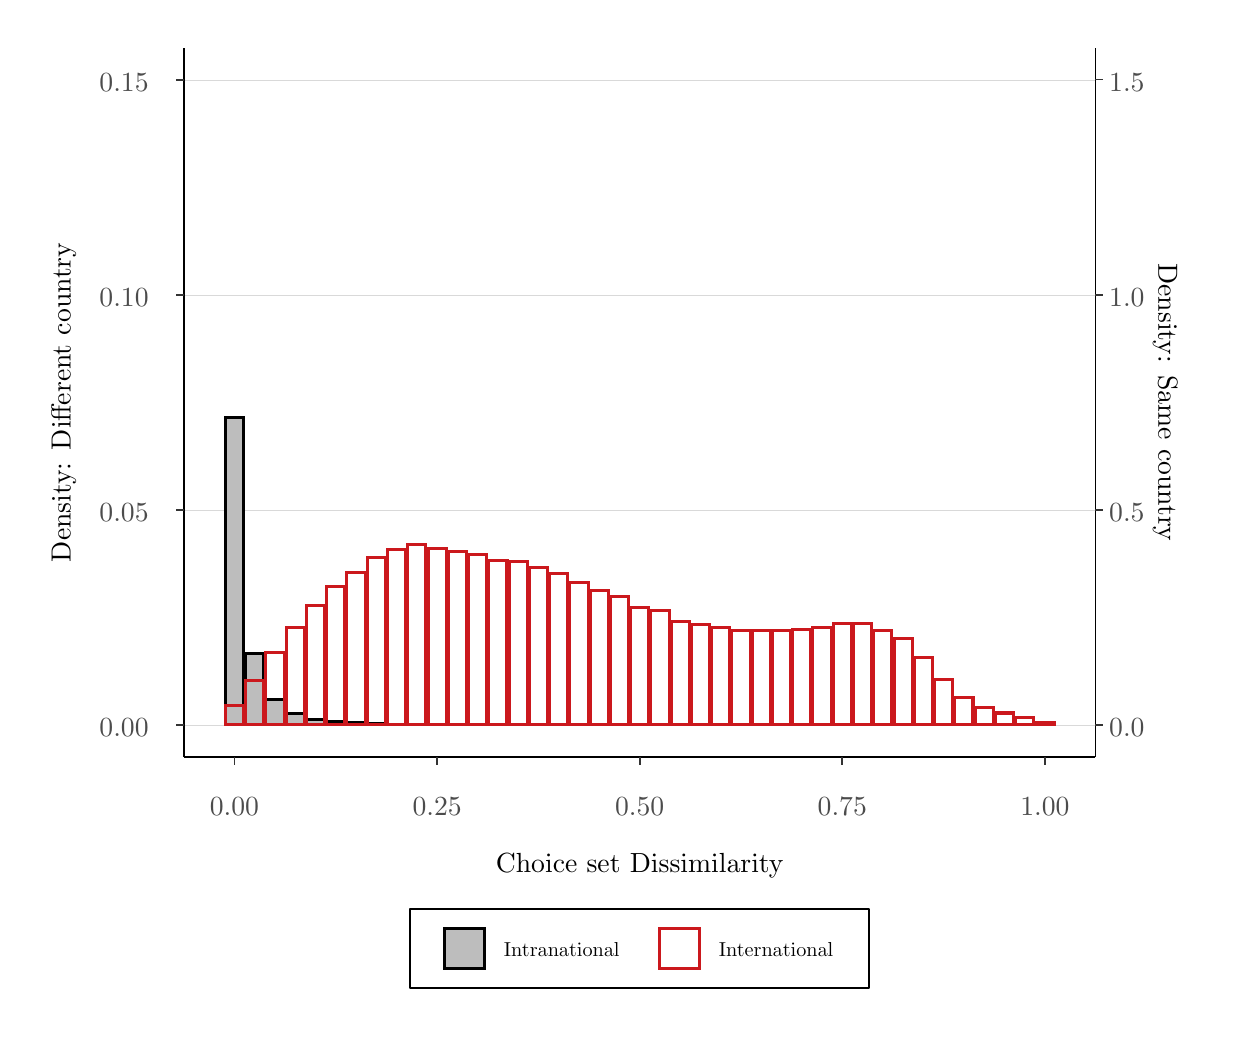
\begin{tikzpicture}[x=1pt,y=1pt]
\definecolor{fillColor}{RGB}{255,255,255}
\path[use as bounding box,fill=fillColor,fill opacity=0.00] (0,0) rectangle (433.62,361.35);
\begin{scope}
\path[clip] (  0.00,  0.00) rectangle (433.62,361.35);
\definecolor{drawColor}{RGB}{255,255,255}
\definecolor{fillColor}{RGB}{255,255,255}

\path[draw=drawColor,line width= 0.6pt,line join=round,line cap=round,fill=fillColor] ( -0.00,  0.00) rectangle (433.62,361.35);
\end{scope}
\begin{scope}
\path[clip] ( 56.47, 97.75) rectangle (385.85,354.12);
\definecolor{drawColor}{RGB}{255,255,255}

\path[draw=drawColor,line width= 0.3pt,line join=round] ( 56.47,148.25) --
	(385.85,148.25);

\path[draw=drawColor,line width= 0.3pt,line join=round] ( 56.47,225.94) --
	(385.85,225.94);

\path[draw=drawColor,line width= 0.3pt,line join=round] ( 56.47,303.62) --
	(385.85,303.62);

\path[draw=drawColor,line width= 0.3pt,line join=round] (111.34, 97.75) --
	(111.34,354.12);

\path[draw=drawColor,line width= 0.3pt,line join=round] (184.55, 97.75) --
	(184.55,354.12);

\path[draw=drawColor,line width= 0.3pt,line join=round] (257.77, 97.75) --
	(257.77,354.12);

\path[draw=drawColor,line width= 0.3pt,line join=round] (330.98, 97.75) --
	(330.98,354.12);
\definecolor{drawColor}{gray}{0.85}

\path[draw=drawColor,line width= 0.1pt,line join=round] ( 56.47,109.40) --
	(385.85,109.40);

\path[draw=drawColor,line width= 0.1pt,line join=round] ( 56.47,187.09) --
	(385.85,187.09);

\path[draw=drawColor,line width= 0.1pt,line join=round] ( 56.47,264.78) --
	(385.85,264.78);

\path[draw=drawColor,line width= 0.1pt,line join=round] ( 56.47,342.47) --
	(385.85,342.47);
\definecolor{drawColor}{RGB}{0,0,0}
\definecolor{fillColor}{gray}{0.74}

\path[draw=drawColor,line width= 1.1pt,line cap=rect,fill=fillColor] ( 71.44,109.40) rectangle ( 78.03,220.56);
\definecolor{drawColor}{RGB}{203,24,29}

\path[draw=drawColor,line width= 1.1pt,line cap=rect] ( 71.44,109.40) rectangle ( 78.03,116.28);
\definecolor{drawColor}{RGB}{0,0,0}

\path[draw=drawColor,line width= 1.1pt,line cap=rect,fill=fillColor] ( 78.76,109.40) rectangle ( 85.35,135.17);
\definecolor{drawColor}{RGB}{203,24,29}

\path[draw=drawColor,line width= 1.1pt,line cap=rect] ( 78.76,109.40) rectangle ( 85.35,125.34);
\definecolor{drawColor}{RGB}{0,0,0}

\path[draw=drawColor,line width= 1.1pt,line cap=rect,fill=fillColor] ( 86.08,109.40) rectangle ( 92.67,118.47);
\definecolor{drawColor}{RGB}{203,24,29}

\path[draw=drawColor,line width= 1.1pt,line cap=rect] ( 86.08,109.40) rectangle ( 92.67,135.67);
\definecolor{drawColor}{RGB}{0,0,0}

\path[draw=drawColor,line width= 1.1pt,line cap=rect,fill=fillColor] ( 93.40,109.40) rectangle ( 99.99,113.56);
\definecolor{drawColor}{RGB}{203,24,29}

\path[draw=drawColor,line width= 1.1pt,line cap=rect] ( 93.40,109.40) rectangle ( 99.99,144.70);
\definecolor{drawColor}{RGB}{0,0,0}

\path[draw=drawColor,line width= 1.1pt,line cap=rect,fill=fillColor] (100.72,109.40) rectangle (107.31,111.51);
\definecolor{drawColor}{RGB}{203,24,29}

\path[draw=drawColor,line width= 1.1pt,line cap=rect] (100.72,109.40) rectangle (107.31,152.42);
\definecolor{drawColor}{RGB}{0,0,0}

\path[draw=drawColor,line width= 1.1pt,line cap=rect,fill=fillColor] (108.04,109.40) rectangle (114.63,110.53);
\definecolor{drawColor}{RGB}{203,24,29}

\path[draw=drawColor,line width= 1.1pt,line cap=rect] (108.04,109.40) rectangle (114.63,159.52);
\definecolor{drawColor}{RGB}{0,0,0}

\path[draw=drawColor,line width= 1.1pt,line cap=rect,fill=fillColor] (115.37,109.40) rectangle (121.96,110.09);
\definecolor{drawColor}{RGB}{203,24,29}

\path[draw=drawColor,line width= 1.1pt,line cap=rect] (115.37,109.40) rectangle (121.96,164.45);
\definecolor{drawColor}{RGB}{0,0,0}

\path[draw=drawColor,line width= 1.1pt,line cap=rect,fill=fillColor] (122.69,109.40) rectangle (129.28,109.82);
\definecolor{drawColor}{RGB}{203,24,29}

\path[draw=drawColor,line width= 1.1pt,line cap=rect] (122.69,109.40) rectangle (129.28,169.93);
\definecolor{drawColor}{RGB}{0,0,0}

\path[draw=drawColor,line width= 1.1pt,line cap=rect,fill=fillColor] (130.01,109.40) rectangle (136.60,109.68);
\definecolor{drawColor}{RGB}{203,24,29}

\path[draw=drawColor,line width= 1.1pt,line cap=rect] (130.01,109.40) rectangle (136.60,172.65);
\definecolor{drawColor}{RGB}{0,0,0}

\path[draw=drawColor,line width= 1.1pt,line cap=rect,fill=fillColor] (137.33,109.40) rectangle (143.92,109.59);
\definecolor{drawColor}{RGB}{203,24,29}

\path[draw=drawColor,line width= 1.1pt,line cap=rect] (137.33,109.40) rectangle (143.92,174.46);
\definecolor{drawColor}{RGB}{0,0,0}

\path[draw=drawColor,line width= 1.1pt,line cap=rect,fill=fillColor] (144.65,109.40) rectangle (151.24,109.54);
\definecolor{drawColor}{RGB}{203,24,29}

\path[draw=drawColor,line width= 1.1pt,line cap=rect] (144.65,109.40) rectangle (151.24,173.11);
\definecolor{drawColor}{RGB}{0,0,0}

\path[draw=drawColor,line width= 1.1pt,line cap=rect,fill=fillColor] (151.97,109.40) rectangle (158.56,109.49);
\definecolor{drawColor}{RGB}{203,24,29}

\path[draw=drawColor,line width= 1.1pt,line cap=rect] (151.97,109.40) rectangle (158.56,172.05);
\definecolor{drawColor}{RGB}{0,0,0}

\path[draw=drawColor,line width= 1.1pt,line cap=rect,fill=fillColor] (159.29,109.40) rectangle (165.88,109.47);
\definecolor{drawColor}{RGB}{203,24,29}

\path[draw=drawColor,line width= 1.1pt,line cap=rect] (159.29,109.40) rectangle (165.88,170.97);
\definecolor{drawColor}{RGB}{0,0,0}

\path[draw=drawColor,line width= 1.1pt,line cap=rect,fill=fillColor] (166.62,109.40) rectangle (173.20,109.45);
\definecolor{drawColor}{RGB}{203,24,29}

\path[draw=drawColor,line width= 1.1pt,line cap=rect] (166.62,109.40) rectangle (173.20,168.69);
\definecolor{drawColor}{RGB}{0,0,0}

\path[draw=drawColor,line width= 1.1pt,line cap=rect,fill=fillColor] (173.94,109.40) rectangle (180.53,109.42);
\definecolor{drawColor}{RGB}{203,24,29}

\path[draw=drawColor,line width= 1.1pt,line cap=rect] (173.94,109.40) rectangle (180.53,168.29);
\definecolor{drawColor}{RGB}{0,0,0}

\path[draw=drawColor,line width= 1.1pt,line cap=rect,fill=fillColor] (181.26,109.40) rectangle (187.85,109.42);
\definecolor{drawColor}{RGB}{203,24,29}

\path[draw=drawColor,line width= 1.1pt,line cap=rect] (181.26,109.40) rectangle (187.85,166.27);
\definecolor{drawColor}{RGB}{0,0,0}

\path[draw=drawColor,line width= 1.1pt,line cap=rect,fill=fillColor] (188.58,109.40) rectangle (195.17,109.41);
\definecolor{drawColor}{RGB}{203,24,29}

\path[draw=drawColor,line width= 1.1pt,line cap=rect] (188.58,109.40) rectangle (195.17,163.97);
\definecolor{drawColor}{RGB}{0,0,0}

\path[draw=drawColor,line width= 1.1pt,line cap=rect,fill=fillColor] (195.90,109.40) rectangle (202.49,109.41);
\definecolor{drawColor}{RGB}{203,24,29}

\path[draw=drawColor,line width= 1.1pt,line cap=rect] (195.90,109.40) rectangle (202.49,161.01);
\definecolor{drawColor}{RGB}{0,0,0}

\path[draw=drawColor,line width= 1.1pt,line cap=rect,fill=fillColor] (203.22,109.40) rectangle (209.81,109.40);
\definecolor{drawColor}{RGB}{203,24,29}

\path[draw=drawColor,line width= 1.1pt,line cap=rect] (203.22,109.40) rectangle (209.81,158.00);
\definecolor{drawColor}{RGB}{0,0,0}

\path[draw=drawColor,line width= 1.1pt,line cap=rect,fill=fillColor] (210.54,109.40) rectangle (217.13,109.40);
\definecolor{drawColor}{RGB}{203,24,29}

\path[draw=drawColor,line width= 1.1pt,line cap=rect] (210.54,109.40) rectangle (217.13,155.74);
\definecolor{drawColor}{RGB}{0,0,0}

\path[draw=drawColor,line width= 1.1pt,line cap=rect,fill=fillColor] (217.86,109.40) rectangle (224.45,109.40);
\definecolor{drawColor}{RGB}{203,24,29}

\path[draw=drawColor,line width= 1.1pt,line cap=rect] (217.86,109.40) rectangle (224.45,151.80);
\definecolor{drawColor}{RGB}{0,0,0}

\path[draw=drawColor,line width= 1.1pt,line cap=rect,fill=fillColor] (225.19,109.40) rectangle (231.77,109.40);
\definecolor{drawColor}{RGB}{203,24,29}

\path[draw=drawColor,line width= 1.1pt,line cap=rect] (225.19,109.40) rectangle (231.77,150.59);
\definecolor{drawColor}{RGB}{0,0,0}

\path[draw=drawColor,line width= 1.1pt,line cap=rect,fill=fillColor] (232.51,109.40) rectangle (239.10,109.40);
\definecolor{drawColor}{RGB}{203,24,29}

\path[draw=drawColor,line width= 1.1pt,line cap=rect] (232.51,109.40) rectangle (239.10,146.66);
\definecolor{drawColor}{RGB}{0,0,0}

\path[draw=drawColor,line width= 1.1pt,line cap=rect,fill=fillColor] (239.83,109.40) rectangle (246.42,109.40);
\definecolor{drawColor}{RGB}{203,24,29}

\path[draw=drawColor,line width= 1.1pt,line cap=rect] (239.83,109.40) rectangle (246.42,145.78);
\definecolor{drawColor}{RGB}{0,0,0}

\path[draw=drawColor,line width= 1.1pt,line cap=rect,fill=fillColor] (247.15,109.40) rectangle (253.74,109.40);
\definecolor{drawColor}{RGB}{203,24,29}

\path[draw=drawColor,line width= 1.1pt,line cap=rect] (247.15,109.40) rectangle (253.74,144.60);
\definecolor{drawColor}{RGB}{0,0,0}

\path[draw=drawColor,line width= 1.1pt,line cap=rect,fill=fillColor] (254.47,109.40) rectangle (261.06,109.40);
\definecolor{drawColor}{RGB}{203,24,29}

\path[draw=drawColor,line width= 1.1pt,line cap=rect] (254.47,109.40) rectangle (261.06,143.41);
\definecolor{drawColor}{RGB}{0,0,0}

\path[draw=drawColor,line width= 1.1pt,line cap=rect,fill=fillColor] (261.79,109.40) rectangle (268.38,109.40);
\definecolor{drawColor}{RGB}{203,24,29}

\path[draw=drawColor,line width= 1.1pt,line cap=rect] (261.79,109.40) rectangle (268.38,143.62);
\definecolor{drawColor}{RGB}{0,0,0}

\path[draw=drawColor,line width= 1.1pt,line cap=rect,fill=fillColor] (269.11,109.40) rectangle (275.70,109.40);
\definecolor{drawColor}{RGB}{203,24,29}

\path[draw=drawColor,line width= 1.1pt,line cap=rect] (269.11,109.40) rectangle (275.70,143.58);
\definecolor{drawColor}{RGB}{0,0,0}

\path[draw=drawColor,line width= 1.1pt,line cap=rect,fill=fillColor] (276.44,109.40) rectangle (283.02,109.40);
\definecolor{drawColor}{RGB}{203,24,29}

\path[draw=drawColor,line width= 1.1pt,line cap=rect] (276.44,109.40) rectangle (283.02,144.05);
\definecolor{drawColor}{RGB}{0,0,0}

\path[draw=drawColor,line width= 1.1pt,line cap=rect,fill=fillColor] (283.76,109.40) rectangle (290.35,109.40);
\definecolor{drawColor}{RGB}{203,24,29}

\path[draw=drawColor,line width= 1.1pt,line cap=rect] (283.76,109.40) rectangle (290.35,144.47);
\definecolor{drawColor}{RGB}{0,0,0}

\path[draw=drawColor,line width= 1.1pt,line cap=rect,fill=fillColor] (291.08,109.40) rectangle (297.67,109.40);
\definecolor{drawColor}{RGB}{203,24,29}

\path[draw=drawColor,line width= 1.1pt,line cap=rect] (291.08,109.40) rectangle (297.67,146.16);
\definecolor{drawColor}{RGB}{0,0,0}

\path[draw=drawColor,line width= 1.1pt,line cap=rect,fill=fillColor] (298.40,109.40) rectangle (304.99,109.40);
\definecolor{drawColor}{RGB}{203,24,29}

\path[draw=drawColor,line width= 1.1pt,line cap=rect] (298.40,109.40) rectangle (304.99,145.92);
\definecolor{drawColor}{RGB}{0,0,0}

\path[draw=drawColor,line width= 1.1pt,line cap=rect,fill=fillColor] (305.72,109.40) rectangle (312.31,109.40);
\definecolor{drawColor}{RGB}{203,24,29}

\path[draw=drawColor,line width= 1.1pt,line cap=rect] (305.72,109.40) rectangle (312.31,143.65);

\path[draw=drawColor,line width= 1.1pt,line cap=rect] (313.04,109.40) rectangle (319.63,140.66);

\path[draw=drawColor,line width= 1.1pt,line cap=rect] (320.36,109.40) rectangle (326.95,133.74);

\path[draw=drawColor,line width= 1.1pt,line cap=rect] (327.68,109.40) rectangle (334.27,125.96);

\path[draw=drawColor,line width= 1.1pt,line cap=rect] (335.01,109.40) rectangle (341.59,119.45);

\path[draw=drawColor,line width= 1.1pt,line cap=rect] (342.33,109.40) rectangle (348.92,115.71);

\path[draw=drawColor,line width= 1.1pt,line cap=rect] (349.65,109.40) rectangle (356.24,113.70);

\path[draw=drawColor,line width= 1.1pt,line cap=rect] (356.97,109.40) rectangle (363.56,112.07);

\path[draw=drawColor,line width= 1.1pt,line cap=rect] (364.29,109.40) rectangle (370.88,110.18);
\end{scope}
\begin{scope}
\path[clip] (  0.00,  0.00) rectangle (433.62,361.35);
\definecolor{drawColor}{RGB}{0,0,0}

\path[draw=drawColor,line width= 0.6pt,line join=round] ( 56.47, 97.75) --
	( 56.47,354.12);
\end{scope}
\begin{scope}
\path[clip] (  0.00,  0.00) rectangle (433.62,361.35);
\definecolor{drawColor}{gray}{0.30}

\node[text=drawColor,anchor=base east,inner sep=0pt, outer sep=0pt, scale=  1.00] at ( 43.72,105.27) {0.00};

\node[text=drawColor,anchor=base east,inner sep=0pt, outer sep=0pt, scale=  1.00] at ( 43.72,182.96) {0.05};

\node[text=drawColor,anchor=base east,inner sep=0pt, outer sep=0pt, scale=  1.00] at ( 43.72,260.65) {0.10};

\node[text=drawColor,anchor=base east,inner sep=0pt, outer sep=0pt, scale=  1.00] at ( 43.72,338.34) {0.15};
\end{scope}
\begin{scope}
\path[clip] (  0.00,  0.00) rectangle (433.62,361.35);
\definecolor{drawColor}{gray}{0.20}

\path[draw=drawColor,line width= 0.6pt,line join=round] ( 53.72,109.40) --
	( 56.47,109.40);

\path[draw=drawColor,line width= 0.6pt,line join=round] ( 53.72,187.09) --
	( 56.47,187.09);

\path[draw=drawColor,line width= 0.6pt,line join=round] ( 53.72,264.78) --
	( 56.47,264.78);

\path[draw=drawColor,line width= 0.6pt,line join=round] ( 53.72,342.47) --
	( 56.47,342.47);
\end{scope}
\begin{scope}
\path[clip] (  0.00,  0.00) rectangle (433.62,361.35);
\definecolor{drawColor}{RGB}{0,0,0}

\path[draw=drawColor,line width= 0.6pt,line join=round] (385.85, 97.75) --
	(385.85,354.12);
\end{scope}
\begin{scope}
\path[clip] (  0.00,  0.00) rectangle (433.62,361.35);
\definecolor{drawColor}{gray}{0.20}

\path[draw=drawColor,line width= 0.6pt,line join=round] (385.85,109.30) --
	(388.60,109.30);

\path[draw=drawColor,line width= 0.6pt,line join=round] (385.85,187.06) --
	(388.60,187.06);

\path[draw=drawColor,line width= 0.6pt,line join=round] (385.85,264.82) --
	(388.60,264.82);

\path[draw=drawColor,line width= 0.6pt,line join=round] (385.85,342.57) --
	(388.60,342.57);
\end{scope}
\begin{scope}
\path[clip] (  0.00,  0.00) rectangle (433.62,361.35);
\definecolor{drawColor}{gray}{0.30}

\node[text=drawColor,anchor=base west,inner sep=0pt, outer sep=0pt, scale=  1.00] at (390.80,105.16) {0.0};

\node[text=drawColor,anchor=base west,inner sep=0pt, outer sep=0pt, scale=  1.00] at (390.80,182.92) {0.5};

\node[text=drawColor,anchor=base west,inner sep=0pt, outer sep=0pt, scale=  1.00] at (390.80,260.68) {1.0};

\node[text=drawColor,anchor=base west,inner sep=0pt, outer sep=0pt, scale=  1.00] at (390.80,338.44) {1.5};
\end{scope}
\begin{scope}
\path[clip] (  0.00,  0.00) rectangle (433.62,361.35);
\definecolor{drawColor}{RGB}{0,0,0}

\path[draw=drawColor,line width= 0.6pt,line join=round] ( 56.47, 97.75) --
	(385.85, 97.75);
\end{scope}
\begin{scope}
\path[clip] (  0.00,  0.00) rectangle (433.62,361.35);
\definecolor{drawColor}{gray}{0.20}

\path[draw=drawColor,line width= 0.6pt,line join=round] ( 74.73, 95.00) --
	( 74.73, 97.75);

\path[draw=drawColor,line width= 0.6pt,line join=round] (147.95, 95.00) --
	(147.95, 97.75);

\path[draw=drawColor,line width= 0.6pt,line join=round] (221.16, 95.00) --
	(221.16, 97.75);

\path[draw=drawColor,line width= 0.6pt,line join=round] (294.37, 95.00) --
	(294.37, 97.75);

\path[draw=drawColor,line width= 0.6pt,line join=round] (367.59, 95.00) --
	(367.59, 97.75);
\end{scope}
\begin{scope}
\path[clip] (  0.00,  0.00) rectangle (433.62,361.35);
\definecolor{drawColor}{gray}{0.30}

\node[text=drawColor,anchor=base,inner sep=0pt, outer sep=0pt, scale=  1.00] at ( 74.73, 76.73) {0.00};

\node[text=drawColor,anchor=base,inner sep=0pt, outer sep=0pt, scale=  1.00] at (147.95, 76.73) {0.25};

\node[text=drawColor,anchor=base,inner sep=0pt, outer sep=0pt, scale=  1.00] at (221.16, 76.73) {0.50};

\node[text=drawColor,anchor=base,inner sep=0pt, outer sep=0pt, scale=  1.00] at (294.37, 76.73) {0.75};

\node[text=drawColor,anchor=base,inner sep=0pt, outer sep=0pt, scale=  1.00] at (367.59, 76.73) {1.00};
\end{scope}
\begin{scope}
\path[clip] (  0.00,  0.00) rectangle (433.62,361.35);
\definecolor{drawColor}{RGB}{0,0,0}

\node[text=drawColor,anchor=base,inner sep=0pt, outer sep=0pt, scale=  1.00] at (221.16, 56.13) {Choice set Dissimilarity};
\end{scope}
\begin{scope}
\path[clip] (  0.00,  0.00) rectangle (433.62,361.35);
\definecolor{drawColor}{RGB}{0,0,0}

\node[text=drawColor,rotate= 90.00,anchor=base,inner sep=0pt, outer sep=0pt, scale=  1.00] at ( 15.49,225.94) {Density: Different country};
\end{scope}
\begin{scope}
\path[clip] (  0.00,  0.00) rectangle (433.62,361.35);
\definecolor{drawColor}{RGB}{0,0,0}

\node[text=drawColor,rotate=-90.00,anchor=base,inner sep=0pt, outer sep=0pt, scale=  1.00] at (408.57,225.94) {Density: Same country};
\end{scope}
\begin{scope}
\path[clip] (  0.00,  0.00) rectangle (433.62,361.35);
\definecolor{drawColor}{RGB}{0,0,0}
\definecolor{fillColor}{RGB}{255,255,255}

\path[draw=drawColor,line width= 0.6pt,line join=round,line cap=round,fill=fillColor] (138.25, 14.45) rectangle (304.07, 42.80);
\end{scope}
\begin{scope}
\path[clip] (  0.00,  0.00) rectangle (433.62,361.35);

\path[] (149.25, 19.95) rectangle (166.60, 37.30);
\end{scope}
\begin{scope}
\path[clip] (  0.00,  0.00) rectangle (433.62,361.35);
\definecolor{drawColor}{RGB}{0,0,0}
\definecolor{fillColor}{gray}{0.74}

\path[draw=drawColor,line width= 1.1pt,line cap=rect,fill=fillColor] (150.67, 21.38) rectangle (165.17, 35.88);
\end{scope}
\begin{scope}
\path[clip] (  0.00,  0.00) rectangle (433.62,361.35);

\path[] (226.90, 19.95) rectangle (244.24, 37.30);
\end{scope}
\begin{scope}
\path[clip] (  0.00,  0.00) rectangle (433.62,361.35);
\definecolor{drawColor}{RGB}{203,24,29}

\path[draw=drawColor,line width= 1.1pt,line cap=rect] (228.32, 21.38) rectangle (242.82, 35.88);
\end{scope}
\begin{scope}
\path[clip] (  0.00,  0.00) rectangle (433.62,361.35);
\definecolor{drawColor}{RGB}{0,0,0}

\node[text=drawColor,anchor=base west,inner sep=0pt, outer sep=0pt, scale=  0.73] at (172.10, 25.60) {Intranational};
\end{scope}
\begin{scope}
\path[clip] (  0.00,  0.00) rectangle (433.62,361.35);
\definecolor{drawColor}{RGB}{0,0,0}

\node[text=drawColor,anchor=base west,inner sep=0pt, outer sep=0pt, scale=  0.73] at (249.74, 25.60) {International};
\end{scope}
\end{tikzpicture}
}
    \end{subfigure}
     \parbox{\textwidth}{
        \begin{spacing}{1} 
            {\footnotesize 
            \textit{Notes}: This figure plots the distribution for the count-based dissimilarity measures across NUTS2-region pairs. The unit of observation is at the product category-region $l$-region $l'$-year level. The grey bars plot the distribution for intranational pairs and the red bars do the same for international pairs. Panel (a) plots the count-based dissimilarity measure and panel (b) plots the expenditure-based dissimilarity measure for product varieties. Panel (c) and (d) do the same for firm-level dissimilarity measures. Note that panel (d) has two y-axes: the left y-axis scales with the different country region pairs and the right y-axis scales with the same country region pairs. }
        \end{spacing}}
\end{figure} 
To control for increased geographic differences across international region pairs, we re-estimate equation \ref{eq:border_effect_prices} for the four dissimilarity measures: 
\begin{linenomath*}
\begin{equation}\label{eq:border_effect_barcodes}
    y_{pll',t} = \beta B_{ll'} + \gamma d_{ll'} + \theta_l + \theta_{l'} +
                    \lambda_{p,t} + \varepsilon_{p(i)ll',t}
\end{equation}
\end{linenomath*}
where $y_{pll',t} = \left\{N^{B,ll'}_{p,t},\lambda^{B,ll'}_{p,t},N^{F,ll'}_{p,t},\lambda^{F,ll'}_{p,t}\right\}$. As before, we include a border dummy $B_{ll'}$ which is one when NUTS2-region $l$ and NUTS2-region $l'$ are an international region pair and zero otherwise, $d_{ll'}$, the log of the population-weighted distance between NUTS2-region $l$ and NUTS2-region $l'$ and product category-year $\lambda_{p,t}$ and region fixed effects $\theta_l$ and $\theta_{l'}$. 

Table \ref{tab: border_effects_choice} presents the baseline OLS estimates. First, columns (1), (4), (7) and (10) show that more distant regions are characterized by larger choice set differences independent of the dissimilarity measure used. Even if the distance coefficient considerably drops when conditioning on national borders in columns (2), (5), (7) and (11), it remains positive and significantly different from zero. For instance, column (2) shows that a 100\% increase in distance or a doubling of the distance between two regions increases choice set differences in terms of product variety counts by 5.1\%. Second, in line with Figures \ref{fig: redform_bar_c} and \ref{fig: redform_bar_e} we estimate large border effects for the product variety level dissimilarity measures. Within product category - years, column (2) illustrates that the overlap in choice sets decreases by more than 71.7ppt for international pairs. In other words, intranational pairs have more than five times as many product varieties in common compared to international pairs.\footnote{This number is obtained from the following calculation: $\frac{0.178+0.717}{0.178} = 5.028$} The border effect for expenditure-based choice set differences in column (5) is similarly estimated at 73.8ppt. Although there is cross-country heterogeneity in the average choice set dissimilarity for intranational pairs, columns (3) and (6) confirm that the border effects are positive, independent of the chosen baseline country. Third, the border effects for the dissimilarity measures at the firm level are lower relative to the ones at the product variety level. Column (8) shows that intranational pairs have more than five times as many firms in common compared to international pairs.\footnote{This number is obtained from the following calculation: $\frac{0.149+0.649}{0.149} = 5.35$} However, consistent with Figure \ref{fig: redform_firm_e} the firm-level border effects in terms of expenditure are substantially lower. Column (10) illustrates that consumers across international pairs spend on average more than 50\% on product varieties provided by firms common to both regions. Nevertheless, large differences remain as consumers in intranational pairs spend on average more than 97\% on product varieties provided by common firms. Columns (9) and (12) confirm that these results are robust to accounting for cross-country heterogeneity in differences for intranational pairs. \footnote{Throughout the analysis, Belgium seems to consistently have lower estimated border effects. The country dummy indicates that variation across Belgian region pairs is consistently higher compared to other countries. Therefore, the border effects from the Belgian perspective are lower.}

\begin{landscape}
    \begin{table}
        \centering
        \caption{Border effect: Choice set dissimilarity}
        \label{tab: border_effects_choice}
        \begin{spacing}{1.1}
            \scalebox{0.8}{
            \begin{tabular}{lcccccccccccc} \toprule
                & \multicolumn{3}{c}{$N^{B,ll'}_{p,t}$} & \multicolumn{3}{c}{$\lambda^{B,ll'}_{p,t}$}   
                & \multicolumn{3}{c}{$N^{F,ll'}_{p,t}$} & \multicolumn{3}{c}{$\lambda^{F,ll'}_{p,t}$} \\ 
                \cmidrule(lr){2-4} \cmidrule(lr){5-7} \cmidrule(lr){8-10} \cmidrule(lr){11-13}
                $y_{p(i)ll',t}$ & (1) & (2) & (3) & (4) & (5) & (6) & (7) & (8) & (9) & (10) & (11) & (12) \\ 
                \midrule
                $d_{ll'}$&$.426^{***}$&$.051^{***}$&$.058^{***}$&$.449^{***}$&$.062^{***}$&$.068^{***}$&$.376^{***}$&$.037^{***}$&$.048^{***}$&$.255^{***}$&$.035^{***}$&$.043^{***}$\\
&$(.009)$&$(.003)$&$(.002)$&$(.01)$&$(.003)$&$(.002)$&$(.008)$&$(.003)$&$(.002)$&$(.006)$&$(.003)$&$(.002)$\\
$B_{ll'}$&&$.717^{***}$&$.767^{***}$&&$.738^{***}$&$.778^{***}$&&$.649^{***}$&$.754^{***}$&&$.421^{***}$&$.474^{***}$\\
&&$(.003)$&$(.004)$&&$(.003)$&$(.004)$&&$(.004)$&$(.004)$&&$(.004)$&$(.004)$\\
$\mathbbm{1}\left(c(l) = c(l') = \text{BEL}\right)$&&&$.285^{***}$&&&$.251^{***}$&&&$.398^{***}$&&&$.362^{***}$\\
&&&$(.009)$&&&$(.009)$&&&$(.008)$&&&$(.008)$\\
$\mathbbm{1}\left(c(l) = c(l') = \text{FRA}\right)$&&&$.037^{***}$&&&$.002$&&&$.147^{***}$&&&$-.005^{*}$\\
&&&$(.007)$&&&$(.008)$&&&$(.008)$&&&$(.008)$\\
$\mathbbm{1}\left(c(l) = c(l') = \text{NLD}\right)$&&&$.138^{***}$&&&$.16^{***}$&&&$.256^{***}$&&&$.221^{***}$\\
&&&$(.007)$&&&$(.009)$&&&$(.007)$&&&$(.007)$\\
\midrule
$\theta_{l}$&$\checkmark$&$\checkmark$&$\checkmark$&$\checkmark$&$\checkmark$&$\checkmark$&$\checkmark$&$\checkmark$&$\checkmark$&$\checkmark$&$\checkmark$&$\checkmark$\\
$\theta_{l'}$&$\checkmark$&$\checkmark$&$\checkmark$&$\checkmark$&$\checkmark$&$\checkmark$&$\checkmark$&$\checkmark$&$\checkmark$&$\checkmark$&$\checkmark$&$\checkmark$\\
$\lambda_{c(i),t}$&$\checkmark$&$\checkmark$&$\checkmark$&$\checkmark$&$\checkmark$&$\checkmark$&$\checkmark$&$\checkmark$&$\checkmark$&$\checkmark$&$\checkmark$&$\checkmark$\\

$\hat{\mathbb{E}}\left(y_{c(i)ll',t}|\text{same}\right)$&.178&.178&.191&.117&.117&.129&.149&.149&.142&.023&.023&.025\\

$\beta - \gamma_{\text{BEL}}$&-&-&$.482^{***}$&-&-&$.526^{***}$&-&-&$.356^{***}$&-&-&$.112^{***}$\\
$\beta - \gamma_{\text{FRA}}$&-&-&$.73^{***}$&-&-&$.776^{***}$&-&-&$.607^{***}$&-&-&$.479^{***}$\\
$\beta - \gamma_{\text{NLD}}$&-&-&$.629^{***}$&-&-&$.617^{***}$&-&-&$.498^{***}$&-&-&$.253^{***}$\\

Nr. obs&4,627,670&4,627,670&4,627,670&4,627,670&4,627,670&4,627,670&4,627,670&4,627,670&4,627,670&4,627,670&4,627,670&4,627,670\\
$\text{Within R}^2$&0.51&0.94&0.94&0.50&0.91&0.92&0.47&0.88&0.90&0.35&0.64&0.66\\
\bottomrule

            \end{tabular}}
        \end{spacing}
        \parbox{1.2\textwidth}{
        \begin{spacing}{1} 
            {\footnotesize 
            \textit{Notes}: This table presents the OLS estimates from equation \label{eq:border_effect_barcodes}. Columns (1) - (3) and columns (4) - (6) estimate the results for the count-based and expenditure dissimilarity measure on the product variety level respectively. Columns (7) - (9) and columns (10) - (12) estimate the results for the count-based and expenditure dissimilarity measure on the firm level respectively. $\hat{\mathbb{E}}\left(y_{p(i)ll',t}|\text{same}\right)$ represents the average value of the left-hand side variable for the same country region pairs in all columns, expect in columns (3), (6), (9) and (12). In these columns, this number represents the average for the baseline country which is Germany. We cluster standard errors at the region pairs and present them in brackets below the coefficient estimates. Reported significance levels are at the $p<0.1^{*}$,$p<0.05^{**}$ and $p<0.01^{***}$ levels.} 
        \end{spacing}}
     \end{table}
\end{landscape}

In line with the results for the standard deviation of log price differences, there is much more heterogeneity across product categories compared to the time series. Figure \ref{fig: app_redform_choice_years} shows that the border effects are very stable for the count- and expenditure-based dissimilarity measures, independent of whether they are computed at the product variety or the firm level. In contrast, Figures \ref{fig: app_redform_choice_bar_cats_n} - \ref{fig: app_redform_choice_firm_cats_e} illustrate that, consistently across all the dissimilarity measures, there is substantial variation across product categories. For instance, Figure \ref{fig: app_redform_choice_firm_cats_e}, which plots the expenditure-based dissimilarity measure at the firm level, shows that choice set overlap varies from a little under 20ppt for deodorants to 60ppt for toilet paper all the while both product categories have a very similar choice set overlap for intranational pairs.